\documentclass[12pt]{article}
\usepackage{graphicx}
\usepackage[section]{placeins}
\usepackage{amsmath}
\usepackage{enumitem}
\usepackage{tcolorbox}
\usepackage{subfigure}
\usepackage{amssymb}
\usepackage{hyperref}
\usepackage{float}


\begin{document}

    \title{
\includegraphics[width=6cm]{images/Pong}\\[2cm]Controlled Procedural Terrain Generation}
    \author{Alfredo Russo}
    \date{A.A. 2021-2022}
    
    \maketitle
    \newpage
    
    \tableofcontents
    \newpage
    

    \section{Introduction}
    % Procedural content generation (PCG) in games is the algorithmic creation of game content with limited or indirect user input. PCG methods are developed and used
    % for a number of different reasons, including saving development time and costs, increasing replayability, allowing for adaptive games, assisting designers 
    % and studying creativity and game design.

    % Some content than others require more time and costs and something like terrain are fundamental in games. 
    % Terrain are usually handmade, it requires a lot of times and resources, so with PGC it is possible to automate the process and help the designer with their work.
    % On of the problem of PCG is the controllability of the content generated so, in order to give more control to designers a technique based on software agent is 
    % used in order to generate terrain. A software agent is an entity capable of understanding surrounding world and taking decision based on this and on the parameters
    % related to it.

    % 1-definition of PCG   2-usage     3-problem solved    4-more control  5-software agent    6-controlled procedural terrain generation using software agent

    Procedural content generation (PCG) in games is the algorithmic creation of game content with limited or indirect user input. PGC has been used over the year 
    for helping designer to create content or create it on the fly, since content creation require a lot of times and resources.

    One of the most important content for games is terrain, it is usually handmade, requiring a lot of work and resources for designer. Even in this case PCG help
    a lot, but don't give so much control to them. In order to avoid this problem a better approach is found, and it is a \textbf{controlled procedural terrain generation
    using software agent}. A software agent is an entity placed on the map capable of understanding the surrounding world taking decision based on that, related to
    the work it was meant to do.

    Starting from this information and thanks to the work of Jonathon Doran and Ian Parberry, \cite{article}, I have developed a controlled procedural terrain generator using software 
    agent, capable of generating an island and add details to it like city, trees and harbors according to the parameters specified by designers for each agent.

    \newpage

    \section{Coastline Agent}
    At beginning there is a big ocean, so all the map points are sea points, then the first agent which work on the map is the coastline agent which is responsible for 
    generating the entire landmass. Its work consist of elevating a number of vertices related to the parameter specified by the designer or subdivide itself in two agents
    until a single agent work with a small number of vertices. How much small the number of vertices can be decided by designers.

    \subsection{Agent parameter}
    To a coastline agent are associated some information like the number of vertices it has to work with and a preferred direction. In order to store this information is used
    a struct which represents an entity of the coastline agent. 

    \begin{itemize}
        \item \textbf{startingFromMapCenter:} this is a boolean value which can be use by designer for specifying if the agent have to start its work from the map center or
        from a random point inside the map.
        \item \textbf{coastlineTokens:} it represents the number of action performable by the agent which consist of move itself to a valid point and elevated this point. 
        The number of tokens is directly related to the number of point the agent have to generate.
        \item \textbf{vertexLimit:} At the beginning, a single coastline agent is responsible for the entire landmass. Since a single agent have to work with a small number
        of vertex, it has to divide itself. This parameter allows designers to decide with how many vertices a single agent have to work with. Until the agent doesn't
        work with a number of vertices less or equal than the value specified it continue to divide itself.
        \item \textbf{maxHeight:} this is a range between [0.03, 1] which represent the max height of the vertices elevated by the agent. Unity terrain has a parameter which 
        represent the maximum height of it (it is possible to change it). For keeping track of the height of the points it is used a heightmap which maps that value inside 
        the range [0, 1].
    \end{itemize}

    The agent divide itself according to the \textbf{vertexLimit} parameter, it is used a queue for storing all the agent which will work on the map. 
    Every time the agent have to be placed on the map, except for the first time, they have to be placed on an already elevated point so a hashset with all coastline point
    (point which height is different from 0) is used. For checking if it is the absolute first time an agent is placed on the map it is used a boolean parameter. 

    \subsection{Agent division}
    The first agent is instantiated giving him a number of vertices equal to all the vertices of the map and a preferred direction. Then thanks to the method \textbf{GetCoastlineAgent},
    it is checked if the agent has a number of vertices on which he has to work, less than the \textbf{vertexLimit} parameter. If not, the agent is divided in two with half
    of vertices than the parent and a randomly preferred direction. Otherwise, the agent is added to the queue previously mentioned.  

    The number of vertices elevated at the end of the work of all agent is given by:

    \begin{equation}
        vertices = coastlineTokens * agentNr
    \end{equation}

    \noindent
    So if the number of vertices that will be elevated is greater than the number of vertices of the map it is impossible to perform the action.

    \subsection{Action}
    Action is a method which duration depends on the number of the agent present in the queue and the number of token for each agent. The first thing done is getting an agent
    from the queue and place it on the map. If it is the first time an agent is placed on the map, the position is computed using the method \textbf{GetStartingPoint}, see 
    section \ref{coastline:StartingPoint}. Otherwise, it is computed with \textbf{FindCoastlinePoint} method, see section \ref{coastline:FindCoastlinePoint}. The location variable is used for keeping
    track the position of the agent.

    Then the agent start searching for nearby valid points using the \textbf{NearPoint} method, which check if the points surrounding location are inside the terrain and if its
    height is equal to 0, so if they are sea points. If no point is found means that all the nearby point are already elevated or not valid,
    so the agent is moved to a random coastline point. When there is at least one valid point near to the agent position, it moves to that point and elevates it with a random
    value between the range [0.03, maxHeight]. If there are more than one point where the agent can move, the position where it will move itself is chosen randomly.

    All the point elevated are added to the hashset in order to easily place the agent on the map and let him searching for a valid point.

    \subsection{Get Starting Point} \label{coastline:StartingPoint}
    The value returned by this method depends on if the designer want the agent work starting from the map center or not, according to \textbf{startingFromMapCenter}
    parameter. If it is, the map center is returned, it is computed starting from the value related to the width and height of the unity terrain. Otherwise, a random
    point inside the map is returned, it will be the center of the landmass generated.

    \subsection{Find Coastline Point} \label{coastline:FindCoastlinePoint}
    This method is used for move the agent to a coastline point near to the sea. It takes in input the agent itself, since the agent is moved according to its preferred
    direction. In order to check if a valid point is found it is used \textbf{CheckNearPoint} method, see section \ref{coastline:CheckNearPoint}.

    The first thing done is to retrieve a random coastline point where to place the agent thanks to \textbf{RandomPoint} method, which easily return a point inside the hashset containing all 
    coastline points. Until a valid point isn't found, the agent is moved in its preferred direction.  Since it is possible that the center of the landmass isn't the center
    of the map, it can happen that agent preferred direction lead it outside the map. If it is the case, the agent is repositioned to the starting point where it was placed and 
    it starts searching in the opposite direction than its preferred one.

    At the end of this method, it is always found a valid point.

    \subsection{Check Near Point} \label{coastline:CheckNearPoint}
    It is used for checking if there is at least one sea point near the location given in input. Starting from the location it checks if the surrounding points are inside
    the terrain and if their height is equal to 0.

    \section{Smoothing Agent}
    Smoothing agent is the one which deals with smoothing points previously elevated by the coastline agent.
    In order to do that it use extended Von Neumann neighborhood, changing the height of the points while it perform a random walk 
    on the map.
    
    \subsection{Agent parameter}
    Like every agent it has parameters that allow designer to lead different results based on it.
    These parameters are:
    \begin{itemize}
        \item \textbf{AgentNr:} it represents the number of agent that will be placed on the map in order to smooth coastline points.
        \item \textbf{returnValue:} this is a value used for understand when the agent have to came back to its starting point. The more the value is high, the more
        the points near the starting point will be smooth. So the agent came back to the starting point periodically and this is useful if some parts of the map need 
        more smoothing than others.
        \item \textbf{smoothingTokens:} it represents, like all other agent, the number of action that the agent can perform. The more the number is high, the more the map will be smooth.
    \end{itemize}

    For speeding up the computation there is another parameter taken by the coastline agent script which is \textbf{coastline points}, so the points where it is possible to place agents.
    This is done because retrieving coastline points (points which height is more than 0) can be performance expensive depending on how much the map is big. 

    \noindent 
    Smoothing agent require terrain to work, so there are all the parameters related to the terrain like \textbf{terrain data}, \textbf{heightmap} and so on \dots

    \noindent
    There is also a parameter called \textbf{neighboringPoint} which is used when the agent have to move itself in an adjacent point.
    
    \noindent
    At the end there is an instance of the smoothing agent in order to let the agent start working after and only after the coastline agent finish its work.

    \subsection{Action}
    This method represents the agent action on the map, but before it can start there are a couple of things to do.
    The first thing is to retrieve all the heights related to map points previously generated by the coastline agent. So the heightmap matrix is filled with this information.
    The second one is to retrieve all the coastline point (the point with heights greater than 0) in order to place the agents on the map. This is done by retrieving the
    related hashset by the coastline agent script in order to avoid useless computation. Furthermore, the complexity of this kind of computation increase with the map size 
    because it is needed to check every point height of the map.
    After these things the action can start.

    Every agent need to be placed on the map but not in a completely random way. The agents have to be placed on a coastline point, so in order to do that a random point is retrieved
    from the hashset which contains them and assigned to the starting point. This point is very important for the smoothing agent because, as previously said, this agent returns
    to its starting point periodically.

    In order to understand when the agent have to return to its starting point it is used a counter (\textbf{count}) originally set to 0;
    
    It is important to track the position of every agent and for this is used a variable called \textbf{location} that is updated during time with the current agent position. 
    At the beginning it is set to the value of the starting point.

    Every agent can perform an action according to the number of the tokens specified. The action can consist of came back to the starting point or change the height of a point
    with extended VonNeumannNeighborhood.

    If the value specified as \textbf{returnValue} is 5, it means that the agent have to came back to the starting point 5 times. In order to compute after how many action the agent
    have to came back, the number of tokens is divided by the returnValue. So if the counter is greater than this value the agent have to came back, the location is set to the
    starting point and the counter is set to 0. Otherwise, the agent can perform its action computing the new height for the point where it is and then update the value in the heightmap.
    After this, the agent move itself on a valid random neighboring point thanks to the \textbf{GetNeighboringPoint} method and the counter is increased by one.

    I choose to use unity coroutine, so every time an agent end its work, the terrain is updated with the new heightmap values.

    \subsection{VonNeumannNeighborhood} \label{section:Von Neumann}
    The VonNeumannNeighborhood method compute the new height of the given point p as the average of points in an extended von Neumann neighborhood of p consisting of the
    four orthogonal map points surrounding p on the elevation grid and the four points beyond these, see figure \ref{fig:vonNeumann}.

    \begin{figure}
        \centering
        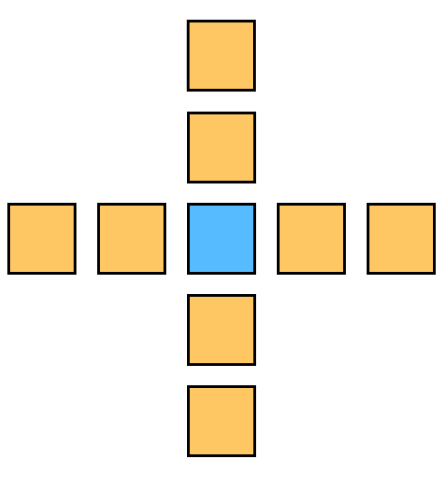
\includegraphics[scale = 0.7]{images/Extended VonNeumannNeighborhood.png}
        \caption{Extended Von Neumann Neighborhood}
        \label{fig:vonNeumann}
    \end{figure}

    \noindent
    A weighted average height is calculated, with the center point given 3 times the weight of the other points. Therefore, nine points with a total weight of eleven are used.
    Starting from this information it is possible to calculate the weight for the central point and the weight for the surrounding points resolving the following equation system:

    \begin{equation}
        \begin{cases}
            x + y = 11
            \\ 3x = y
        \end{cases}
    \end{equation}

    \noindent
    The variable x represents the weight for the central point which is 3 times the other points weight represented by y. So the central point weight is 11/4 and other points weight is 33/4.

    Then the heights of all the points are collected, but it can happen that a surrounding point of location is outside the map. In this case the height considered  is the location one. 
    This choice is done because otherwise the more the points are near to the end of the map, the more their heights will be near to zero, see figure \ref{fig:SmotthingCamparison}.
    
    \begin{figure}
        \centering     %%% not \center
        \subfigure[Height = 0]{\label{fig:Height0}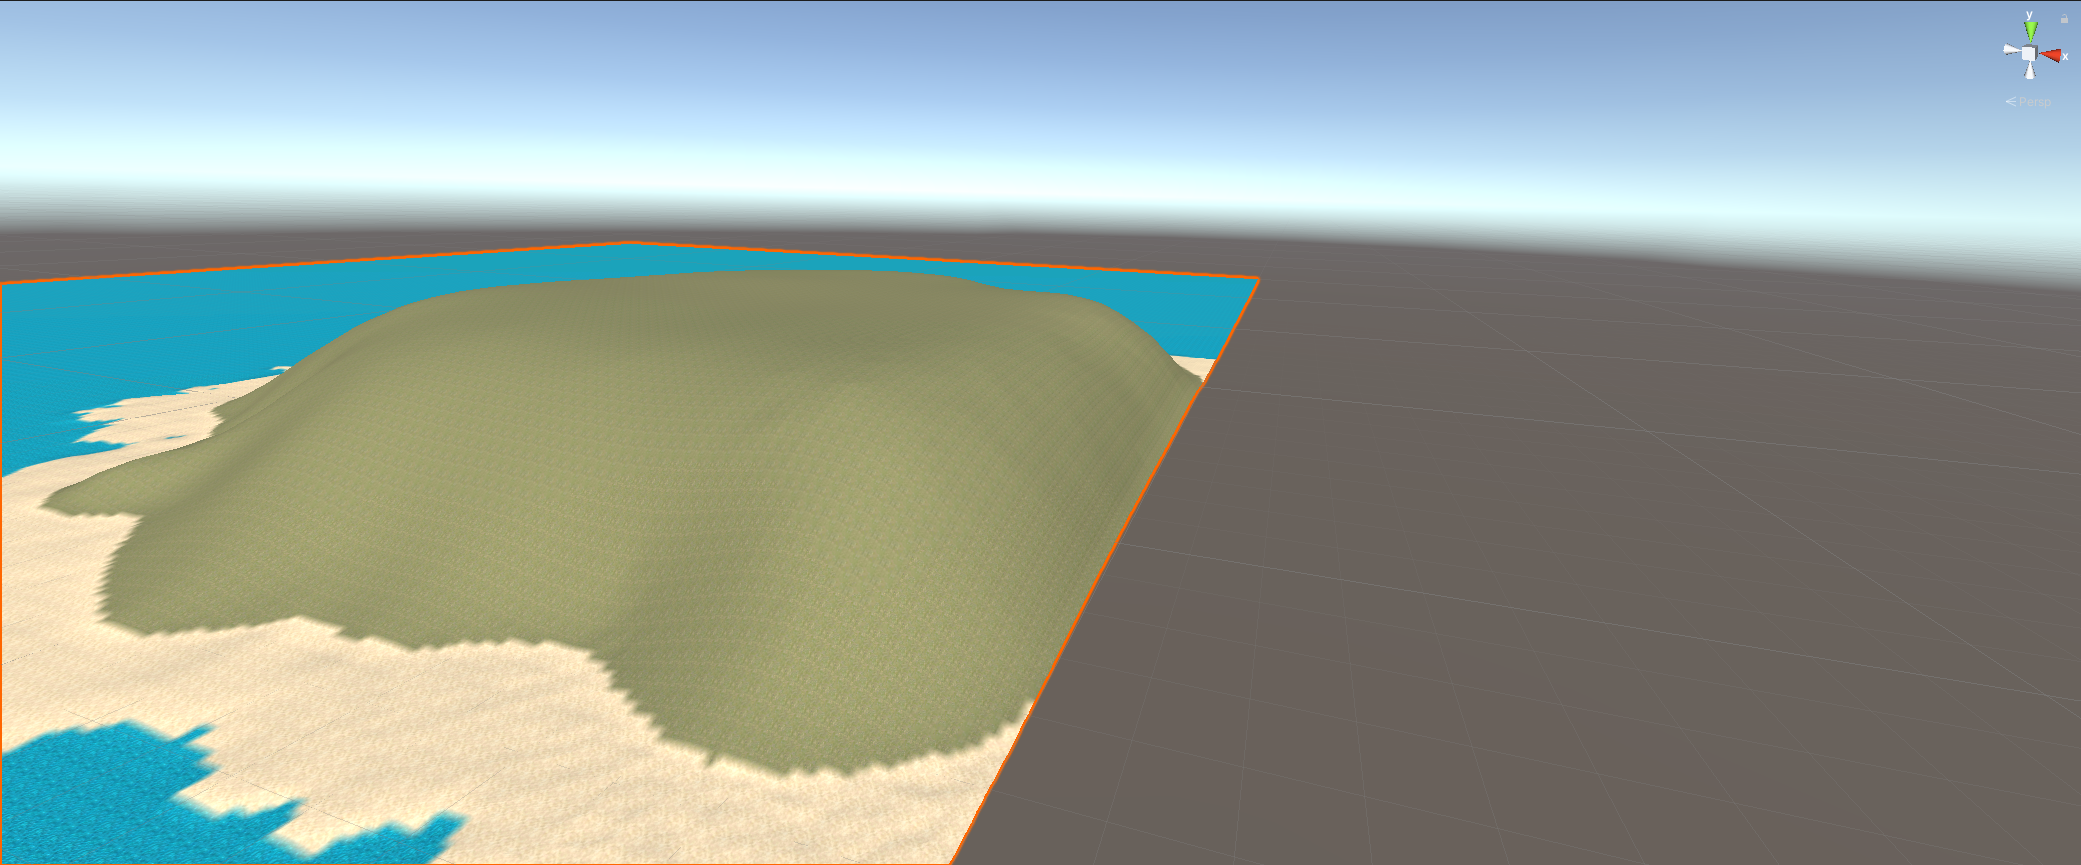
\includegraphics[width=60mm]{images/Smoothing agent height 0}}
        \subfigure[Height = location height]{\label{fig:LocationHeight}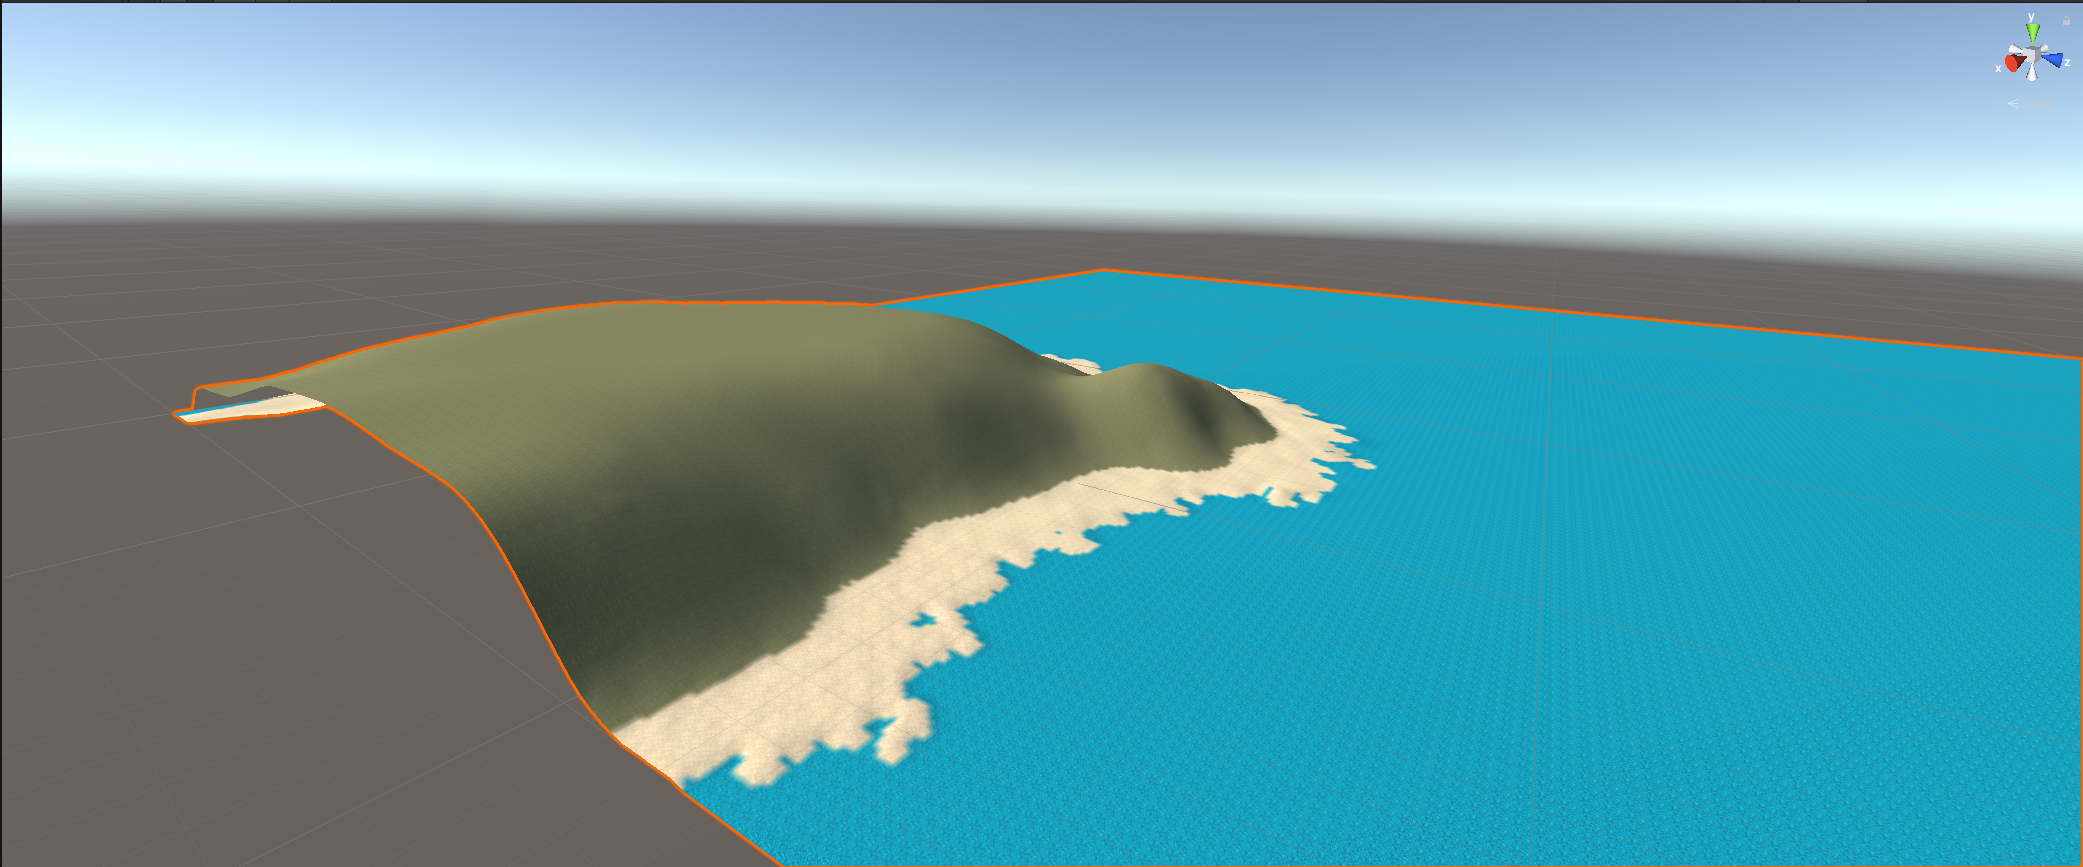
\includegraphics[width=60mm]{images/Smoothing agent height location}}
        \caption{Two different smoothing results.}
        \label{fig:SmotthingCamparison}
    \end{figure}
        
    
    After collected all heights the weighted average height is calculated as follows:

    \begin{equation}
        a = \dfrac{\sum\limits_{i=0}^{9} (W_i * H_i) }{ \sum\limits_{i=0}^{9} W_i }
    \end{equation}

    \noindent
    Where W represent the weight and H represent the height value related to the point. 

    \subsection{GetNeighboringPoint}
    This method takes the current location of the agent and starting from this check if the neighboring point are inside the terrain and then add it to a list. After it is chosen a 
    random point between the valid ones found.

    In order to check if a point is inside the terrain it is used the method called \textbf{IsInsideTerrain} that check if the coordinate of the point are between the range 0 and
    the limit of the map.

    \subsection{Results}
    Below there are some examples of the result achieved and the related configuration about parameters.

    \begin{figure}[H]
        \centering
        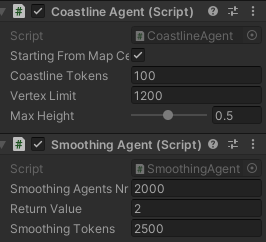
\includegraphics[scale = 0.8]{images/Smoothing agent/256 agenti/Parameters}
        \caption{Parameters used for the following results (256 agents generated).}
        \label{fig:smoothingParam}
    \end{figure}

    \begin{figure}[H]
        \centering
        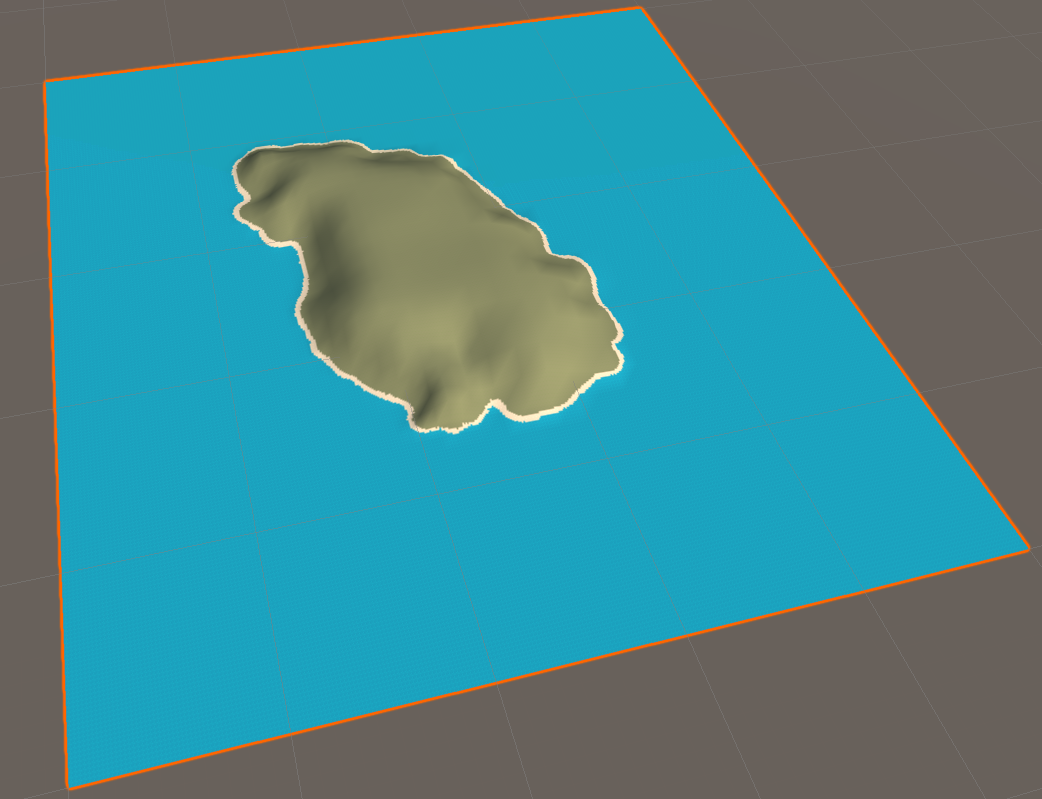
\includegraphics[scale = 0.3]{images/Smoothing agent/256 agenti/1}
        \caption{First results.}
    \end{figure}

    \begin{figure}[H]
        \centering     %%% not \center
        \subfigure[]{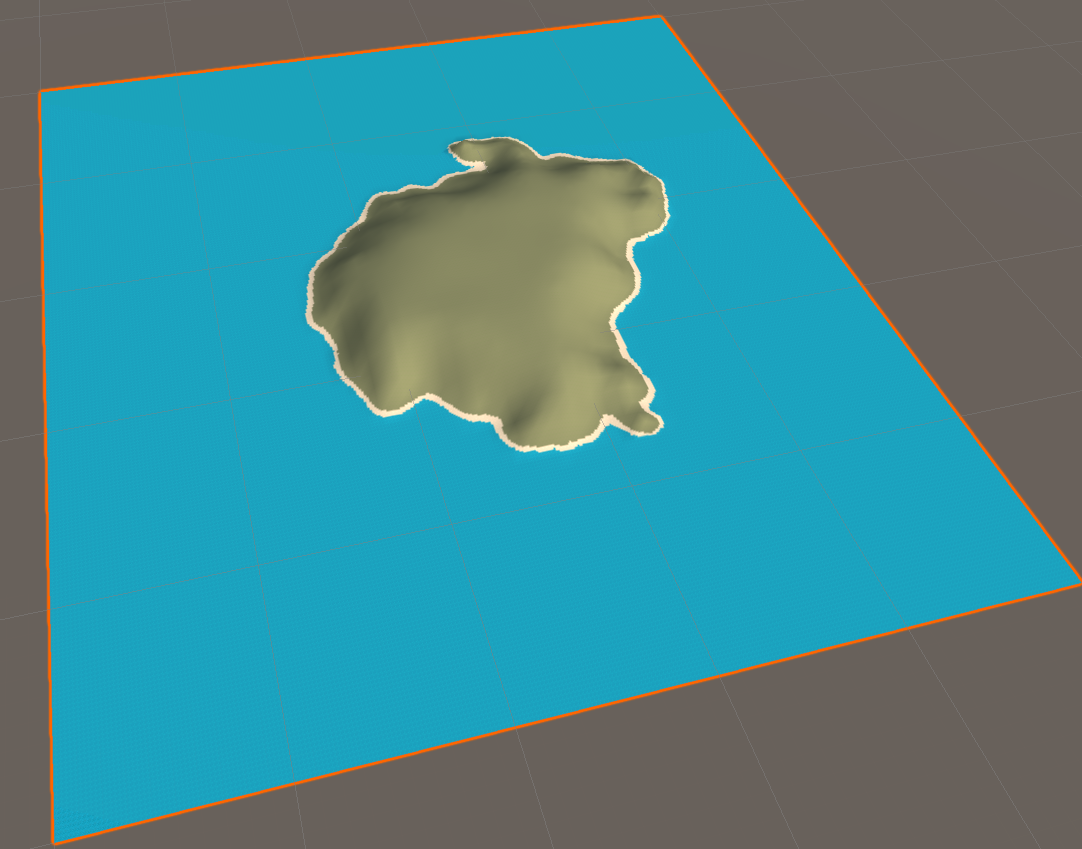
\includegraphics[width=60mm]{images/Smoothing agent/256 agenti/2}}
        \subfigure[]{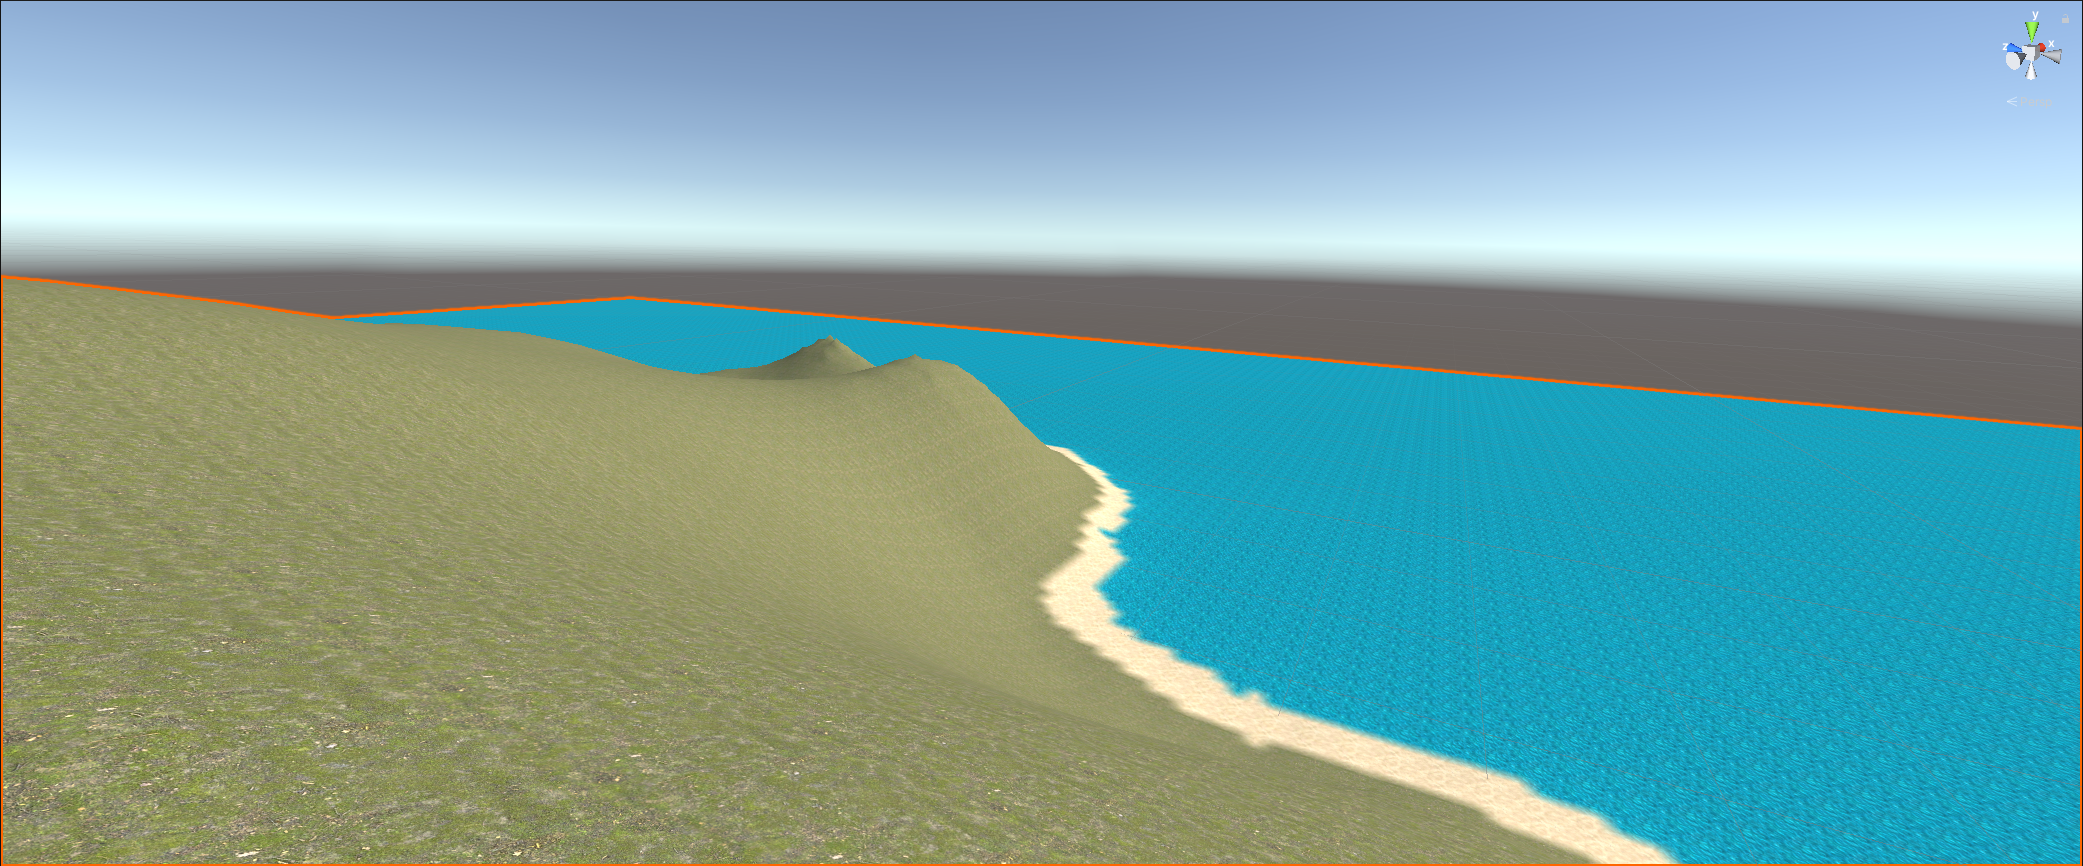
\includegraphics[width=60mm]{images/Smoothing agent/256 agenti/3}}
        \caption{Second results.}
    \end{figure}

    \begin{figure}[H]
        \centering
        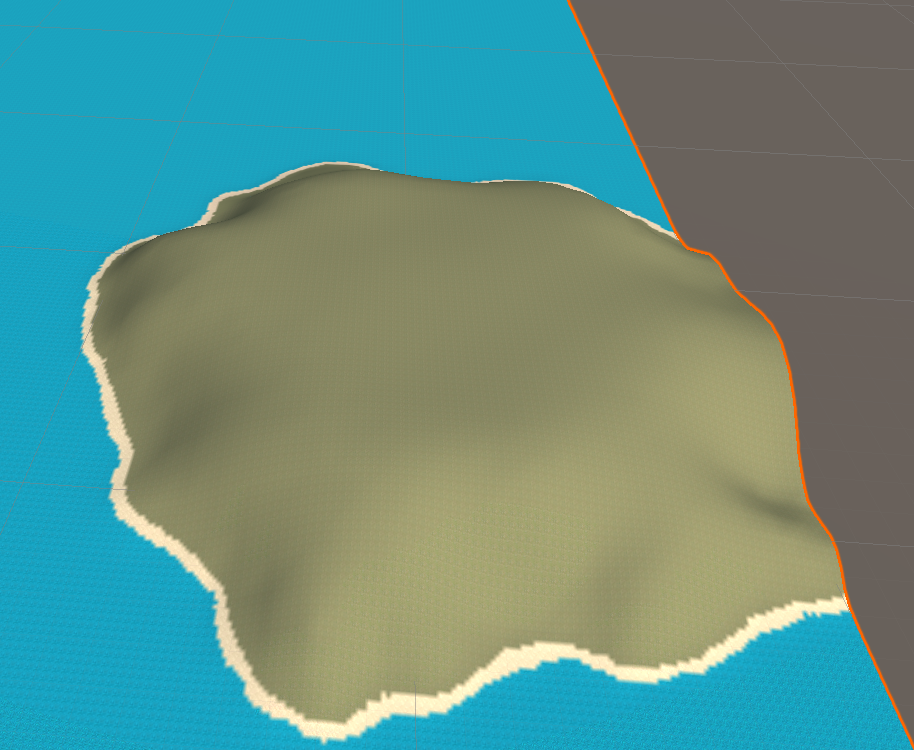
\includegraphics[scale = 0.3]{images/Smoothing agent/256 agenti/4}
        \caption{Third result (it doesn't start from map center).}
    \end{figure}

    \newpage

    \section{Beach Agent}
    This agent start its work after smoothing agent ends its own. In order to do that it is used an instance of the agent that allow to start the action after smoothing agent end its work.
    Beach agent has the work to generate beach according to the parameter chosen by the designer.
    According to this it is possible to obtain a very huge beach all around the coastline or small one in some part of it. It is also possible
    to have flat beach or one that allow fluctuation in its height.

    \subsection{Agent Parameter}
    The beach agent have the following parameter that designer can exploit to generate a different kind of beach:

    \begin{itemize}
        \item \textbf{beachAgentNr:} it represents the number of agent that will work for generating beach.
        \item \textbf{beachTokens:} it is the number of action that each agent have.
        \item \textbf{heightLimit:} it is the altitude limit, when the agent reaches a point higher than the limit specified, it leaves the area
        and move to another random shoreline point.
        \item \textbf{randomWalkSize:} when the agent is placed on a random shoreline point it jumps away from it changing the height of
        the point and smoothing them according to the parameters specified. How long will be its walk is specified by this parameter.
        \item \textbf{awayLimit:} when the agent have to jump away from the coastline it is needed to know how much far.
        So the awayLimit parameter it is really important since it specify that information.
        \item \textbf{beachHeight:} it is a range between [0.003, 0.01[ that represent beach height. Actually, in Unity, we are working with heightmap
        matrix where the heights are mapped inside the range 0-1. So the value previously written have to be multiplied by the maximum height of the 
        unity terrain. If the maximum height of the unity terrain is 100, the range previously specified becomes [0.3, 1[. The more the range is narrow,
        the most the beach will be flat.
    \end{itemize}

    \subsection{Action}
    Before the beach agent action can start, the heightmap matrix have to be filled with the value related to the points' height of unity terrain.
    
    \noindent
    After the smoothing agent action, it can happen that there are points with height between 0 and 0.003 which are neither sea point nor beach point. In 
    order to avoid this behavior a method called \textbf{FlatPoints} is invoked. This method set the height of those points to 0.
    In order to place the agent on the map and replace it when the agent get stuck, a list with all the shoreline points is used and filled thanks to \textbf{GetShorelinePoints}
    method.
    
    Every agent have to be placed on the map, so at the beginning it is retrieved a random shoreline point from the list previously mentioned, and the value is assigned to location
    which represents the current position of the agent that will change over time.

    After the agent is placed on the map it can start its work. The first things to do is to check if the location has an height value greater than the \textbf{heightLimit}.
    If it is, the agent have to be replaced on the map and its location is changed to another random shoreline point.
    
    Then location and its surrounding points are flattened and this means that a random height value between the \textbf{beachHeight} range is assigned
    to them. After these points are smoothed using Von Neumann Neighborhood, see section \ref{section:Von Neumann}.

    Then the agent move itself to a random point away from the coast using \textbf{AwayRandomPoint} method. The new point is stored inside a different variable
    than location since after the agent ends its random walk, it has to came back to the location and move itself to another shoreline point near it.

    Now the agent is ready to start its random walk which duration depends on the parameter \textbf{randomWalkSize}. The agent start to flatten and smooth the away point
    and its neighboring point and only after it moves itself to a valid neighboring point exploiting \textbf{GetNeighboringPoint} method. A point is a valid one if it is 
    inside the map and its height is less than 0.01. It is possible that no valid point near the current position of the agent is found, if it happens means that the 
    agent isn't able to move itself to another point, so its random walk ends. For checking this, it is used a placeholder parameter which is the value -Vector2Int.one.

    When the agent random walk ends, it moves to a new shoreline point near the shoreline point where it was before, assigning the new value to the 
    location variable.

    \subsection{CheckShorelinePoint}
    This method is used by \textbf{GetShorelinePoints} one in order to check if a point is a shoreline one or not. It returns true if the point has a height value
    between the range [0.003, 0.01[. This range was chosen because in this way the points retrieved are point quite close to the sea. Another thing to check by this method is
    if the coordinate of the point plus the away limit are inside the map or not, in order to understand if the agent starting from its position is able to jump away from it.

    \subsection{GetNeighboringPoint}
    This method is used in order to retrieve a position where the agent can move itself exploiting \textbf{GetNeighboringPoints} method which return all
    valid points. If there are no valid points around the location a placeholder value is returned in order to communicate that the agent isn't able
    to move itself.

    \subsection{AwayRandomPoint}
    As previously said, this method allow the agent to jump away from the coast. It add to location a direction multiplied by the \textbf{awayLimit} in order
    to retrieve a point away from the coast and check if it is inside the terrain and its height is less than 0.01. It will be for sure a point away starting
    from the one given in input because every shoreline point can be called like this only if it allows jumping away from it. This check is done by 
    \textbf{GetShorelinePoints} method.

    \subsection{Results}
    Below there are some examples of the result achieved and the related configuration about parameters.

    \begin{figure}[H]
        \centering
        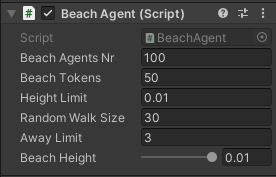
\includegraphics[scale = 0.8]{images/Beach agent/Parameters 1}
        \caption{Parameters used for the following results.}
    \end{figure}

    \begin{figure}[H]
        \centering     %%% not \center
        \subfigure[]{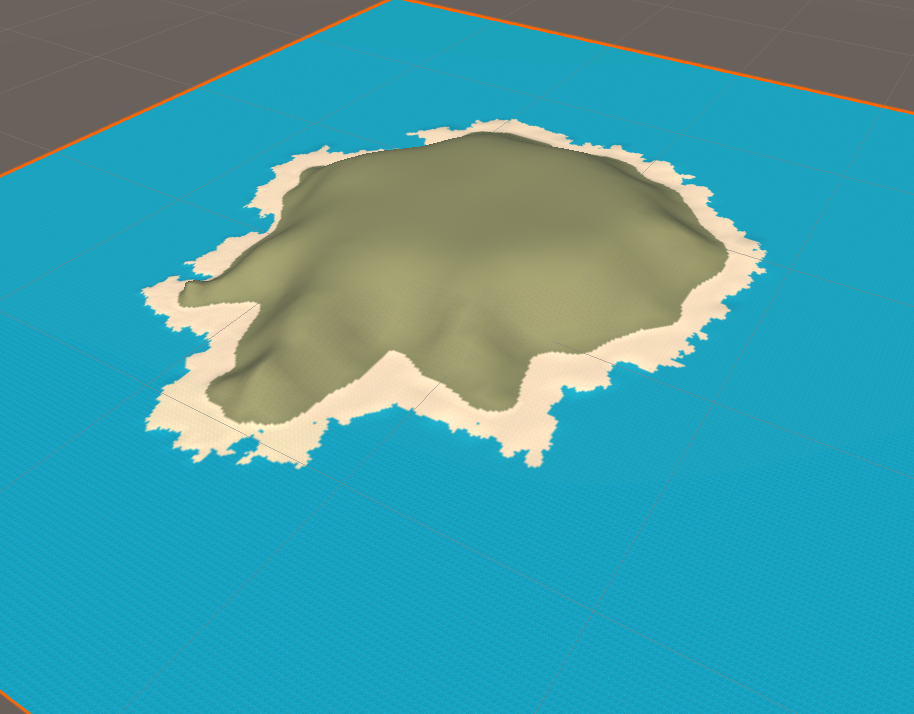
\includegraphics[width=60mm]{images/Beach agent/1}}
        \subfigure[]{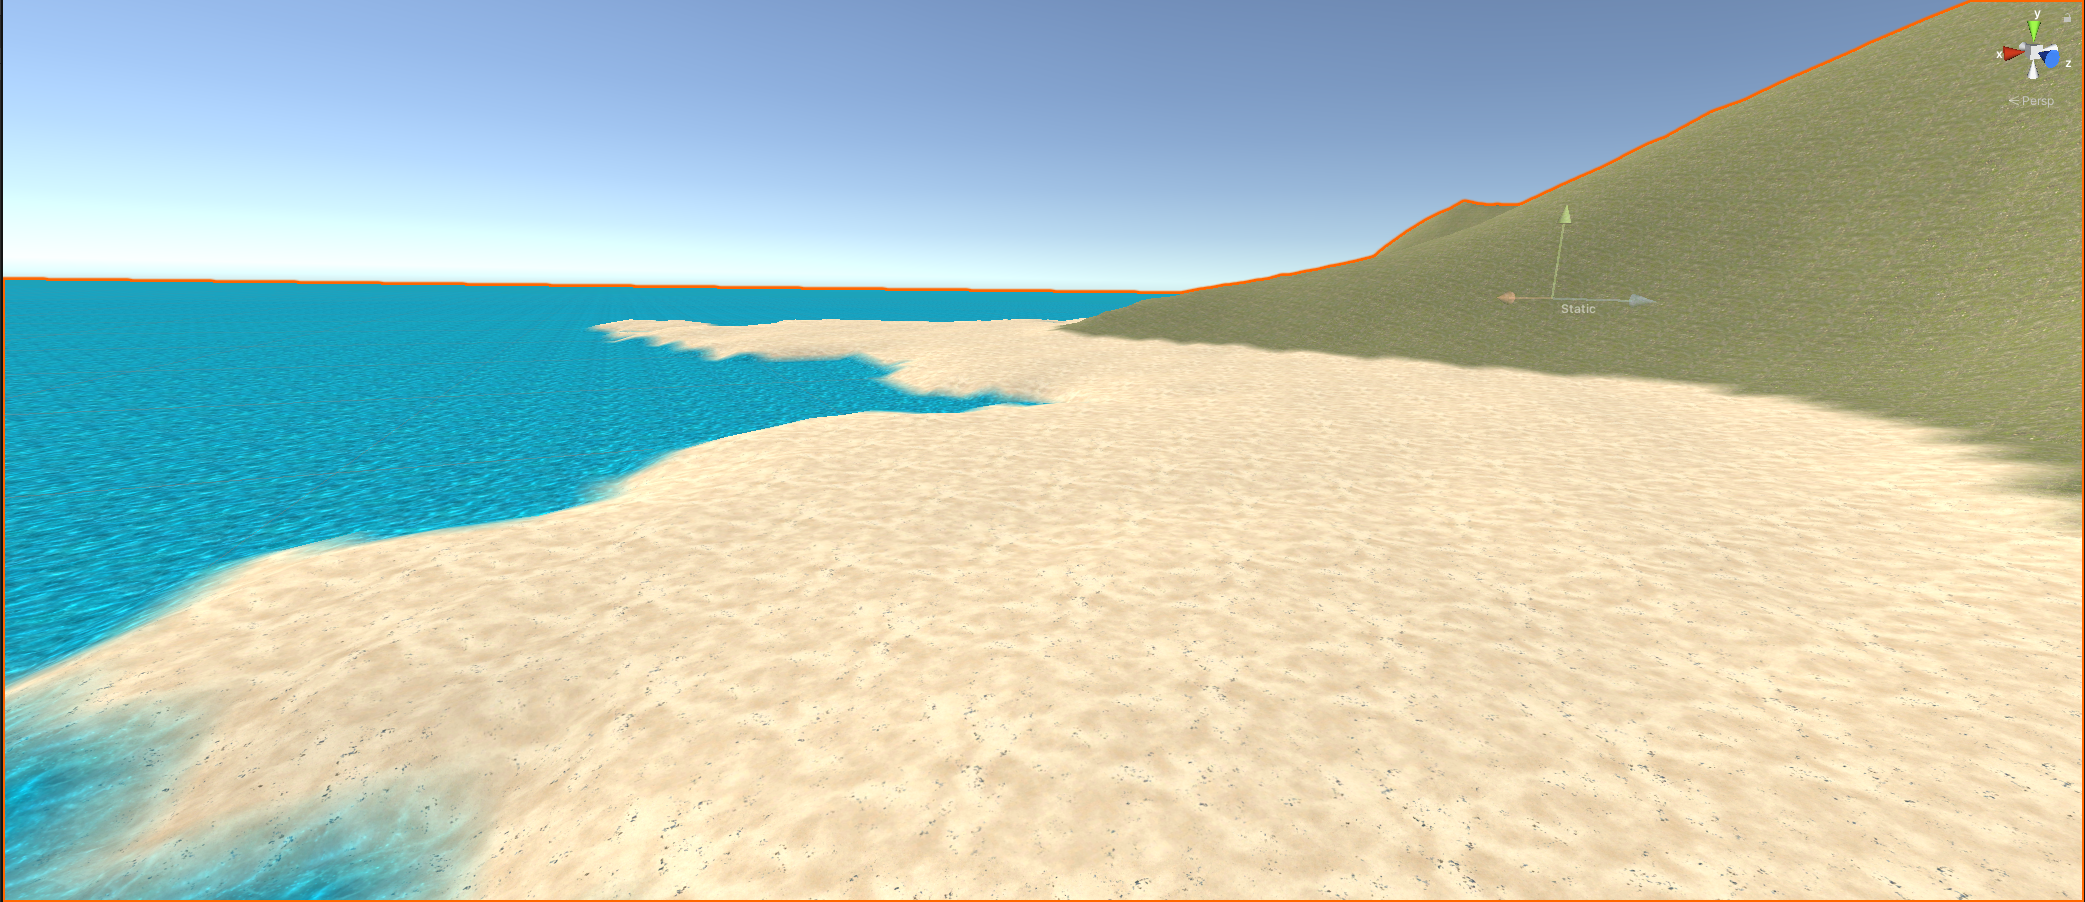
\includegraphics[width=60mm]{images/Beach agent/2}}
        \caption{First results.}
        \label{fig:beachNotFlat}
    \end{figure}

    \begin{figure}[H]
        \centering
        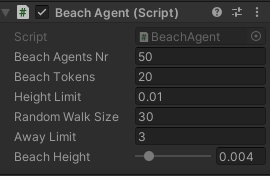
\includegraphics[scale = 0.8]{images/Beach agent/Parameters 2}
        \caption{Parameters used for the following results.}
    \end{figure}

    \begin{figure}[H]
        \centering     %%% not \center
        \subfigure[]{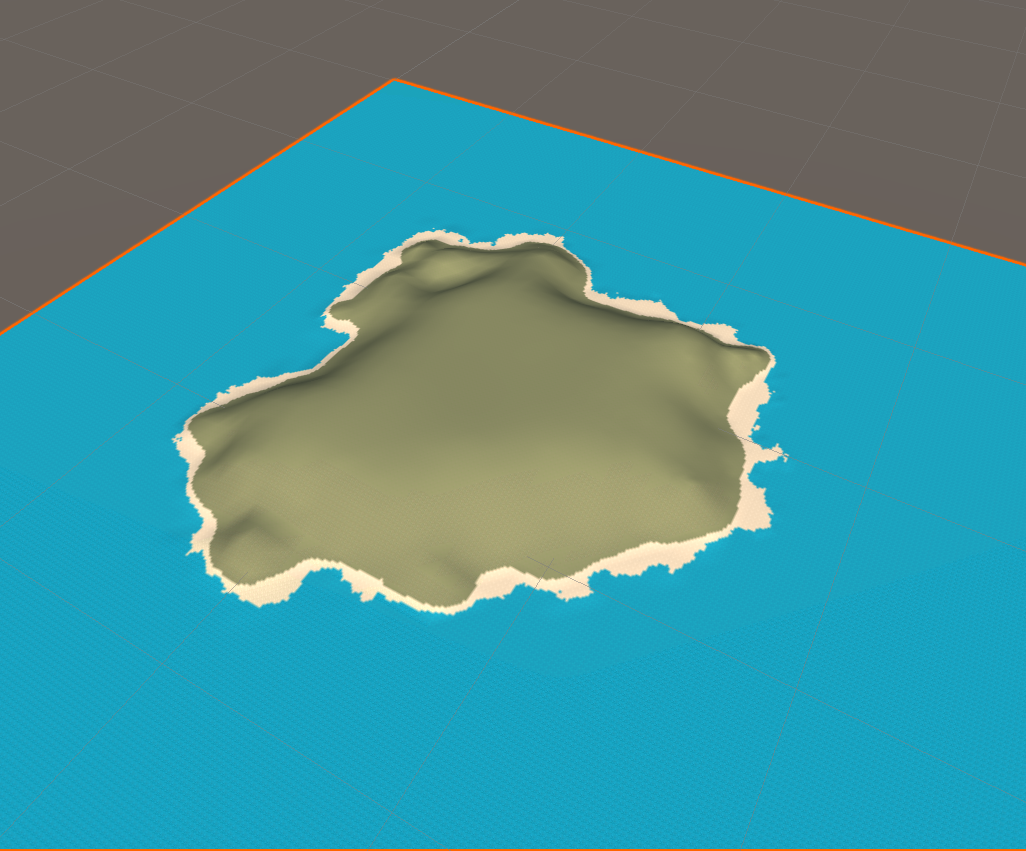
\includegraphics[width=60mm]{images/Beach agent/4}}
        \subfigure[]{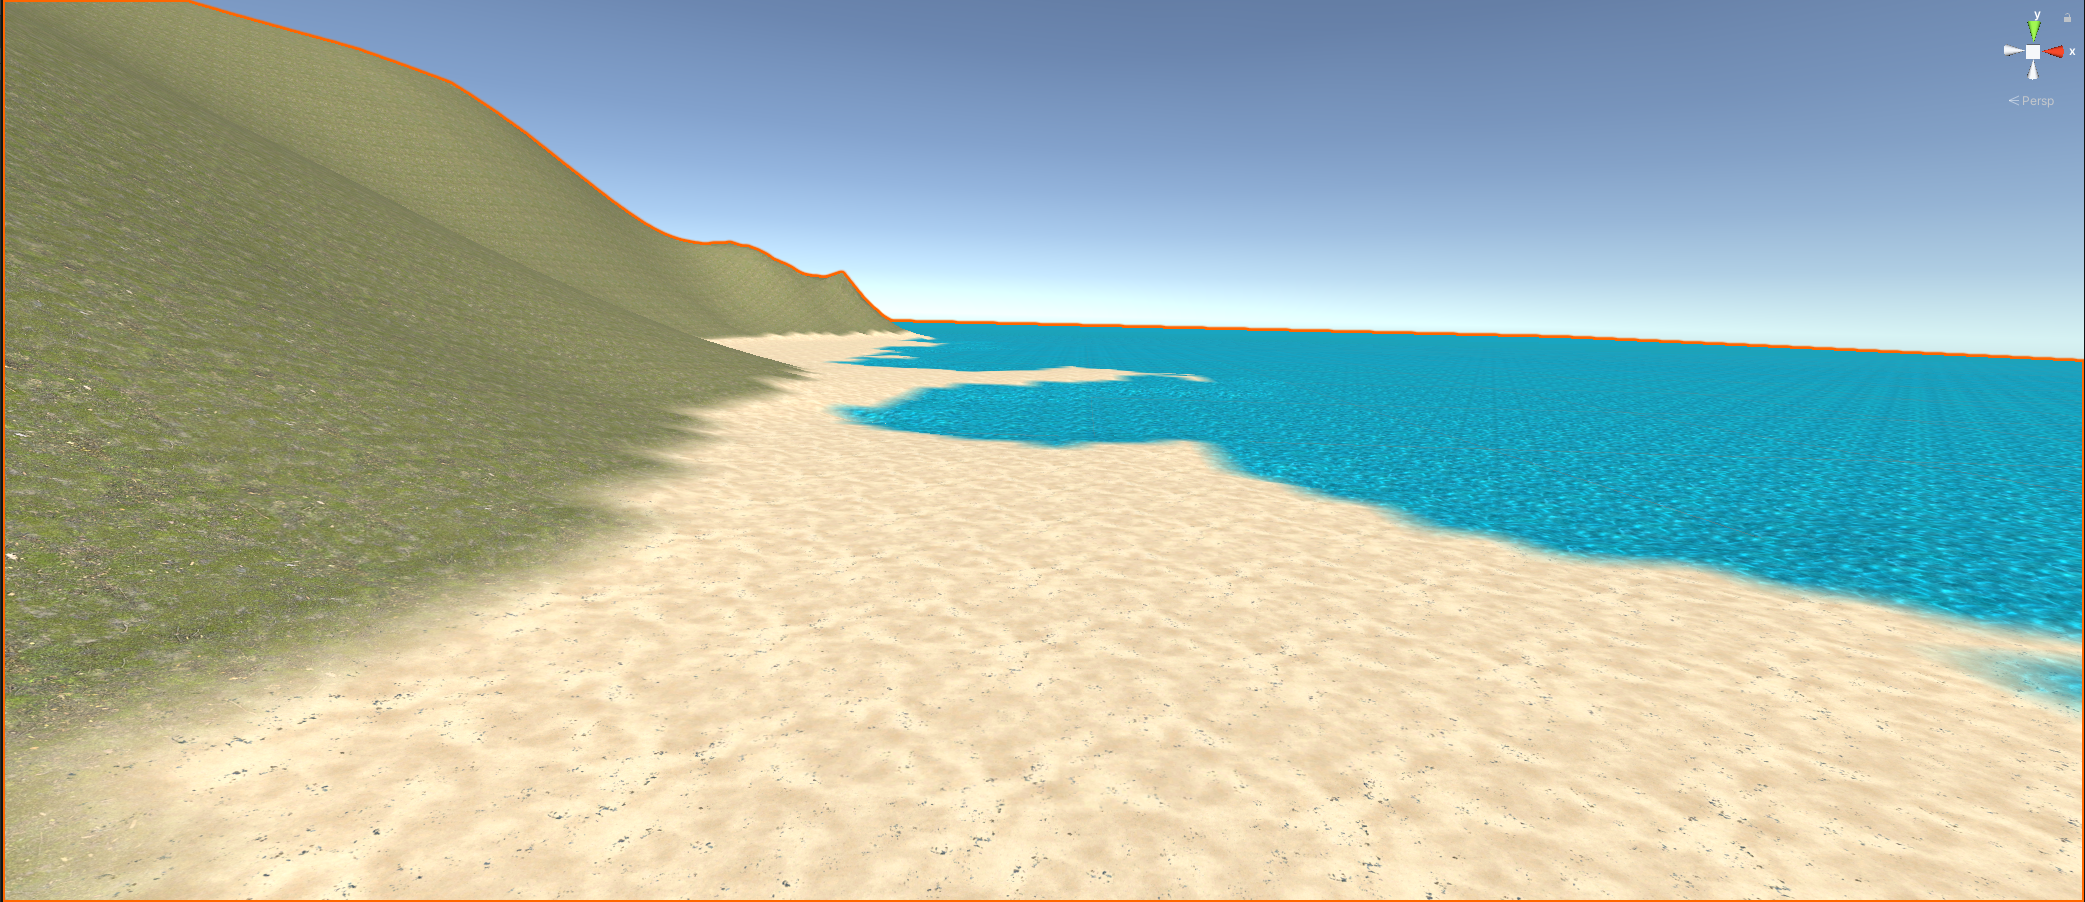
\includegraphics[width=60mm]{images/Beach agent/3}}
        \caption{First results.}
        \label{fig:beachFlat}
    \end{figure}

    As you can see, if the value related to the height of the beach is narrow the beach generated is flat, see \ref{fig:beachFlat}. Otherwise, the beach presents
    some fluctuation, see \ref{fig:beachNotFlat}.

    \newpage

    \section{City Agent}
    City agent is responsible to create roads and houses on the coastline previously created by other agents. This agent can work only if the landmass generated
    is quite flat. 

    \subsection{Agent Parameter}
    \begin{itemize}
        \item \textbf{cityAgentNr:} it is the number of agent which will create the city. Every agent is responsible to create a city zone, the more this 
        number is high, the more the number of city zone will be. Depending on how much the landmass generated is big and how many points where to place roads
        and houses there are, an agent can add details to a zone previously generated by other agents.
        \item \textbf{cityTokens:} it is the number of action performable by the agent. An action for the agent is moving itself to a valid point and place a road 
        and houses according to the following parameter.
        \item \textbf{roadGameObject:} it is the game object that represent the road. It is a simple unity quad.
        \item \textbf{houseGameObject:} the game object that represents house. It is used a simple unity cube with a red material attached on it, there is also a box collider
        in order to perform some checks which will be presented later.
        \item \textbf{gap:} this parameter represents the distance between one house and others. If the gap is equal to 1 the house will be placed side by side
        along the road. Insted if the gap is too high, it can be possible that there is not enough space in order to place houses. After the agent placed a road,
        at least one house is place at the middle of the road, see section \ref{section:CreateHouse}. 
        \item \textbf{roadLength:} it is a range between [5, 20] which specify how long the roads should be. If the length is too high related to the size of the landmass,
        the agent may fail to create a city since there isn't enough space. 
        \item \textbf{numberOfHouse:} This parameter is a dynamic one since it depends on the \textbf{roadLength} and \textbf{gap} specified earlier. In order to achieve this result in unity,
        the editor is changed, and int slider object is used. It requires a variable where the value will be stored, the left value for the slider which is 1, that
        represents the minimum number of house placeable and the right value which represents the maximum number of houses placeable. Actually, the right value parameter depends on
        the road lenght and gap parameters previously mentioned. So in the code there is a dynamic getter for the value \textbf{MaxHouse} which is like following:
        \begin{equation}
            MaxNHouse = \begin{cases} (roadLenght/gap) - 2, & \mbox{if } gap\mbox{ = 1} \\ (roadLenght/gap) - 1, & \mbox{} otherwise\  \end{cases}
        \end{equation}

        The gap equal to 1 means that the house can be placed side by side along the roads. The roads can be orthogonal between them, so the houses, which position is 
        at the end of the road, can be duplicated if the value returned is (roadLength/gap) - 1, see figure \ref{fig:cornerHouse}.
        
        \begin{figure}
            \centering
            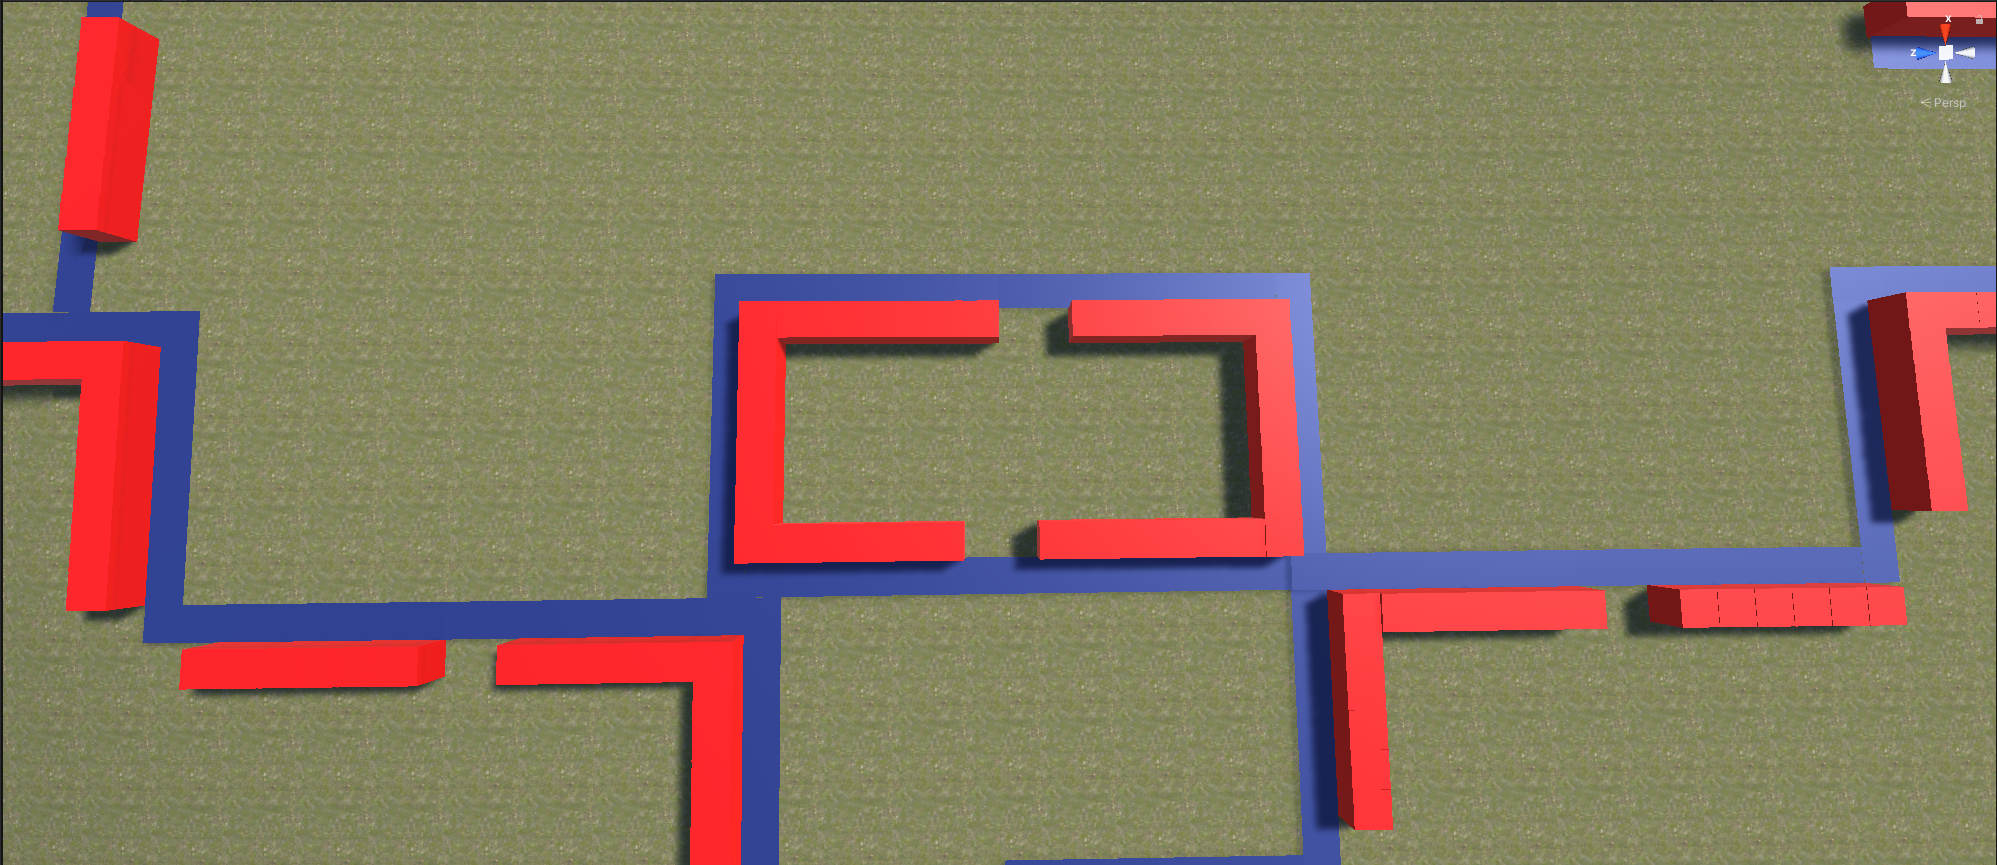
\includegraphics[scale = 0.19]{images/Corner house.png}
            \caption{Corner house}
            \label{fig:cornerHouse}
        \end{figure}
        
    \end{itemize}

    There is an instance of the city agent class since it start working only after the landmass is created, so after beach agent action.

    \subsection{Action} \label{seciton:action}
    As always before the city agent can start, it is needed that all the information about the height are putted inside the heightmap matrix after used
    for different check. There is another important thing to do before the agent can start, it is to retrieve all valid points where the agent can be placed on the
    map, so all valid where the agent can place road and house, see section \ref{section: ValidPoints}.

    Since unity terrain can be placed at every position in the world, it is important to retrieve its position in order to place roads and house at right position on 
    terrain.

    Then every agent have to be placed on the map, in order to do that a random point from the list of all valid points is retrieved and assigned to location variable
    which represent the current position of the agent. In order to not let the agent come back to the previous location when it tries to move itself on the map, that
    position is keep inside \textbf{prevLocation} variable. At beginning this variable is set equal to location, in this way it is possible to understand if the agent
    has just been placed on the map, see section \ref{section:NewLocation}.

    Every agent has a number of tokens to consume which represents the action that can perform. An action for city agent is to place a road and the related number of
    house and then move itself to a valid point. In order to place the road two points are needed, from which a direction is extrapolated. This is done with the methods
    \textbf{CreateRoads} and \textbf{CreateHouse}, see \ref{section:CreateRoad} and \ref{section:CreateHouse}. Since it is used a unity coroutine the agent wait for a frame, and then 
    it moves itself to a new location thanks to \textbf{GetNewLocation} method, see \ref{section:NewLocation}. Before this, the current location of the agent
    is stored inside a temporary variable which value will be the one of the previous location, since the method \textbf{GetNewLocation} need it without being changed.
    If a new location is found the agent move itself to it and the previous location is updated with the value previously stored inside the temporary variable. Otherwise,
    no valid point is found, so the agent can't move itself to another point and its work ends. In order to check if the agent can move to another point or not, the 
    method \textbf{GetNewLocation} return the location given input, so the value returned is like the following:

    \begin{equation}
        location = \begin{cases} location, & \mbox{if } temporaryVariable { = location} \\ newLocation, & \mbox{} otherwise\  \end{cases}
    \end{equation}

    \subsection{Get Valid Points} \label{section: ValidPoints}
    In order to create a city there are some requirements to satisfy. The landmass have to be quite flat and the points considered must not be too steep.
    The first things to do is to considered all the landmass point and distinguish them from the other points like beach and sea one. To perform this task the
    average height of the points which height is greater than 0.01 is considered. So a landmass point is a point which height is greater than the average height plus
    0.05. This value was chosen after some test, it allows to not consider points that are too close to the beach. 

    Then is the time to check if the point consider is too steep or not. In order to do that the method \textbf{CheckStepness} is used. This method, thanks to a
    raycast which is located at position given in input but with a different height, check the angle between the normal of the point and the up vector. If the 
    angle is grater than 7, it means that the point is too steep for considering it as a good point to place roads and houses.
    
    So every map point is checked, and it can be considered a valid one only if its height is greater than the average one plus 0.05 and the angle between the normal 
    and the up vector is less than 7. A list with all valid points is returned.

    \subsection{Get New Location} \label{section:NewLocation}
    This method takes in input the current location of the agent and the previous one. It can happen that the value previously mentioned are the same. This is done in order
    to understand if the agent already started its work, or it has just been placed on the map. So if the agent already started its work, for retrieving position where it
    can move itself the method \textbf{GetCandidates} is used, the one which takes in input the current location of the agent and the previous one. Otherwise, the method
    \textbf{GetCandidates} which takes in input only the location is used. This is done because if the agent has just been placed on the map there are 4 points 
    where it can move itself, otherwise it can move itself only towards 3 points.
    
    Then those points have to be checked, this is done with \textbf{CheckCandidate} method, see \ref{section:CheckCandidate}. At the end it is returned a random point
    between the valid one found or the location given in input if there is neither one valid point where the agent can move itself.
     
    \subsection{Check Candidate} \label{section:CheckCandidate}
    It is used for check if the point considered is a valid one or not. This method takes two input, location which represents where the agent can move itself and 
    previous location which represents the current location of the agent.

    The first thing to do is to check if the location is inside terrain, but this time, unless the others, as upper bound it is used the size of the map minus 1. This is done
    because the point retrieved is a point where the road will be placed, since the houses are placed to the edge of the road considering the border like previously said
    lead to avoid placing houses outside the map. For the same reason the lower bound start from 1 instead of 0, so any point which has 0 inside coordinate isn't a valid one.

    Then it is needed to check the location steepness, this is done thanks to \textbf{CheckSteepness} method previously mentioned, see \ref{seciton:action}.

    Since a road can be placed only by given two points, and it will be placed along all the point between them, it is needed to check if the point along the direction
    from the previous location (current agent position) and location (the possible future agent position) there is something that will make location not 
    a valid point. For every point between location and previous location, it is checked to its right and left and twice its right and left, if there is another point where
    a road is placed. This is done because the house are placed at the edge of the road, so in order to avoid house collision every road need an empty space along
    its edge. So if there is a point to its right or left \textbf{or} twice its right or left, the location considered is not a valid one. Instead, if there is a road to
    its right and left \textbf{and} twice its right and left means that there is a road which will intersect the future one between previous location and location with a 
    90-degree angle, and this is a wanted behavior. When the agent check for a candidate point, the one to its right and left are always with a 90-degree angle. 
    In order to avoid checking left and right points near previous location, since there is almost surely a road to its right or left, checking points start from the 
    following point towards direction.
    
    At the end it is checked if along the point between location and previous location there is already another road.

    \subsection{Create Road} \label{section:CreateRoad}
    This method, starting from the location where the agent is, the previous location and terrain position, place a road on terrain. The first thing done is to retrieve 
    world coordinate (Vector3) of location and previous location from terrain one (Vector2). Then a direction, from previous location to location, is computed as well as the distance
    between them. Before it is possible to instantiate the road it is needed to compute its rotation and scaling. For the rotation it is used the 
    method called \textbf{Quaternion.LookRotation} which take in input the direction in which the road have to look at and the up vector. Then it is computed the Vector3
    related to scaling which the first two coordinates are settled to 1 and the Z one is settled to the length of the road. At this point the road is instantiated on the previous
    location with rotation and scaling previously computed. Then it is translated to middle point between previous and current location and a bit up in order to not have the 
    road colliding with terrain.

    \subsection{Create House} \label{section:CreateHouse}
    It receives in input, as the previous method, the previous and current location and terrain position. Then the world coordinates of previous and current location are 
    computed like the direction from previous to current location. The first house is placed all the times to the middle of the road, so this point is found using the \textbf{Lerp}
    function between previous and current location. Then the rotation is calculated, as previously for the road, with \textbf{Quaternion.LookRotation} method, this time the
    first input is the cross product between the direction vector and the up vector. Since the cross product give back the orthogonal vector between the two in input
    it is retrieved the perpendicular direction than direction. So the house ``will always look'' the roads as well as the forward vector. Thanks to that, the house is
    translated to one unit behind using \textbf{-Vector3.forward}. If the parameter related to the number of house to place is equal to 1 means that the work of the agent ends, 
    otherwise the position for the other house have to be computed. 
    
    Other houses are place first to the right and then to the left of the first one placed, until the number of house which have to be placed is reached. The right direction in which
    the houses have to be places is the same as the direction computed from previous and current location, while left one is the inverse of it. So, starting from the first house position,
    the new position is calculated exploiting the directions previous mentioned according to the gap parameter. Since, as house, it is used a cube, all of them are translated 0.5 upward
    avoiding collision with terrain.

    \subsection{Results}
    Below there are some examples of the result achieved and the related configuration about parameters.

    \begin{figure}[H]
        \centering
        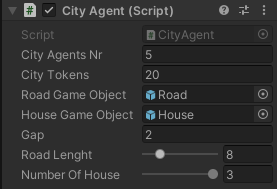
\includegraphics[scale = 0.8]{images/City Agent/1/Parameters}
        \caption{Parameters used for the following results.}
    \end{figure}

    \begin{figure}[H]
        \centering     %%% not \center
        \subfigure[First result]{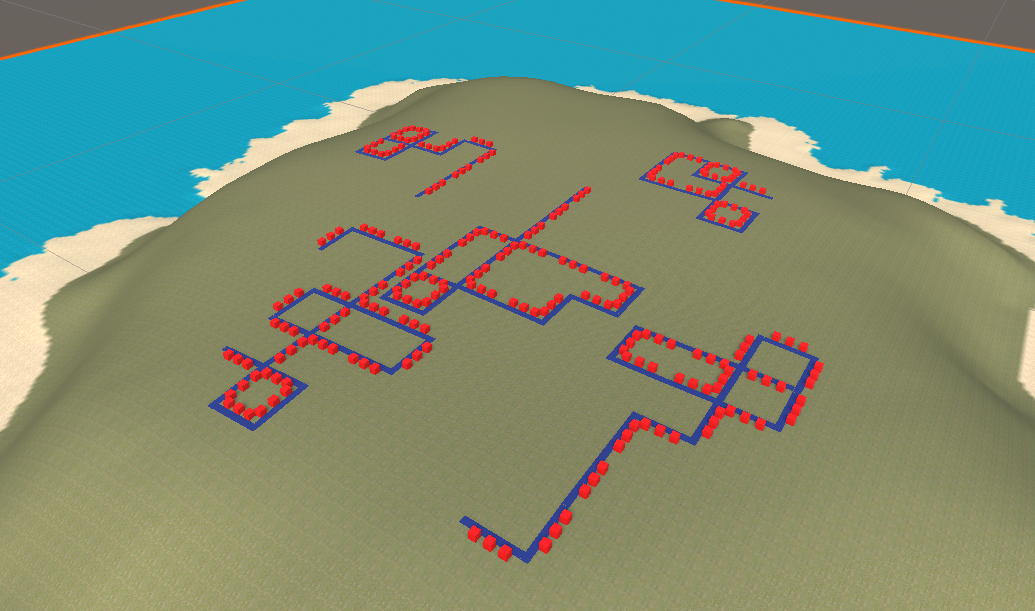
\includegraphics[width=80mm]{images/City Agent/1/1}}
        \subfigure[Second result]{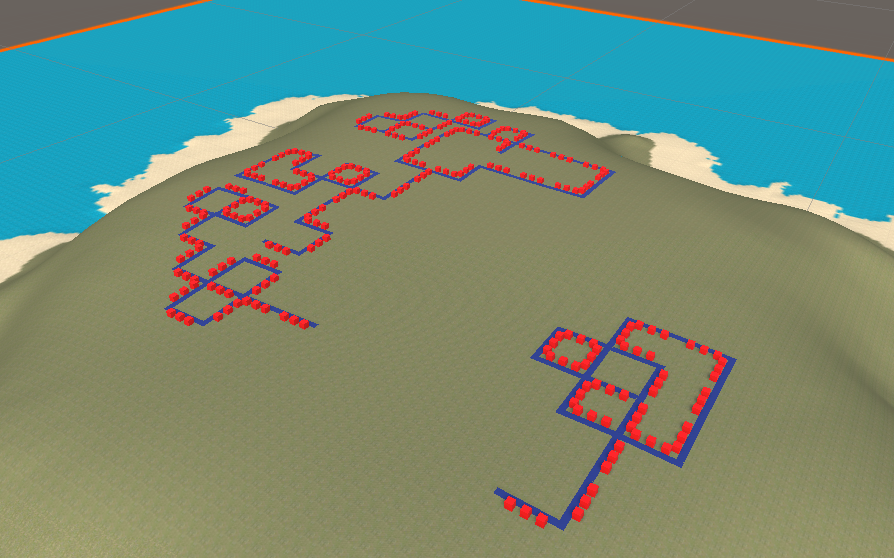
\includegraphics[width=80mm]{images/City Agent/1/2}}
    \end{figure}

    \begin{figure}[H]
        \centering
        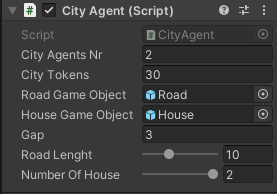
\includegraphics[scale = 0.8]{images/City Agent/2/Parameters}
        \caption{Parameters used for the following results.}
    \end{figure}

    \begin{figure}[H]
        \centering     %%% not \center
        \subfigure[First result]{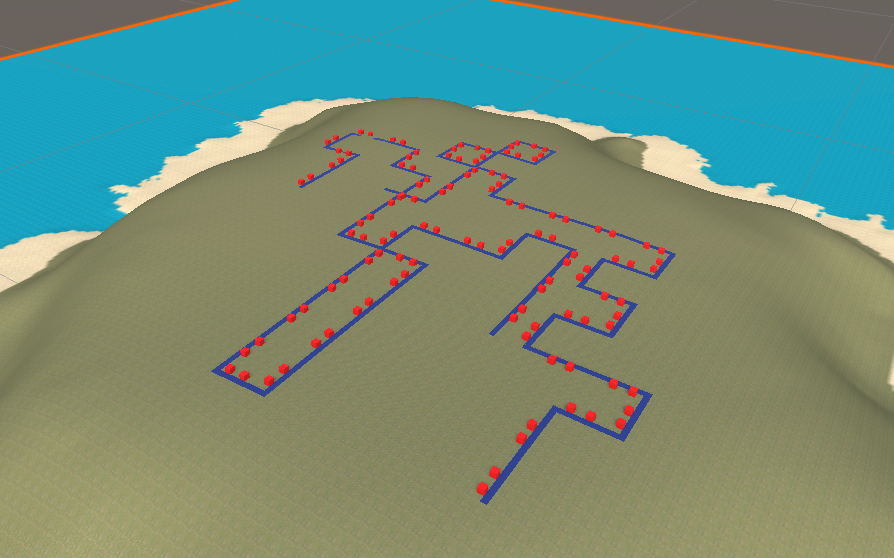
\includegraphics[width=60mm]{images/City Agent/2/1}}
        \subfigure[Second result]{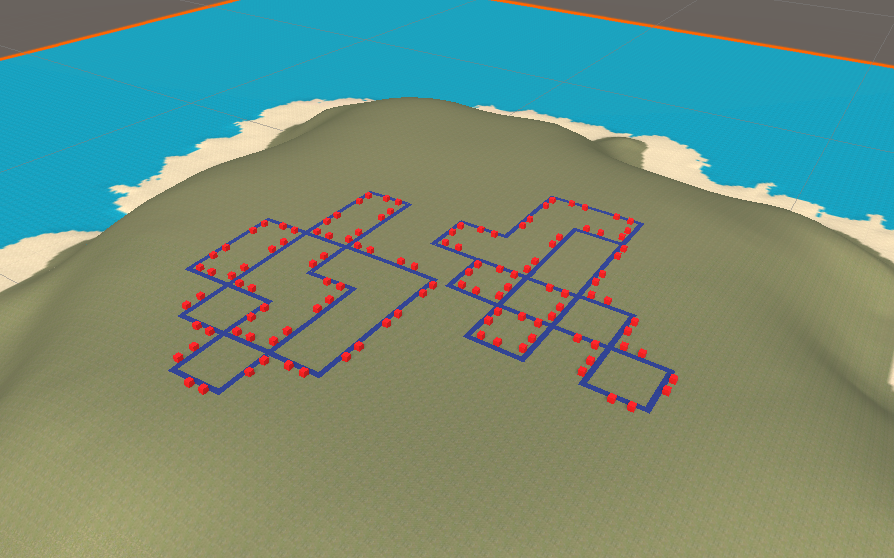
\includegraphics[width=60mm]{images/City Agent/2/2}}
        \subfigure[Third result]{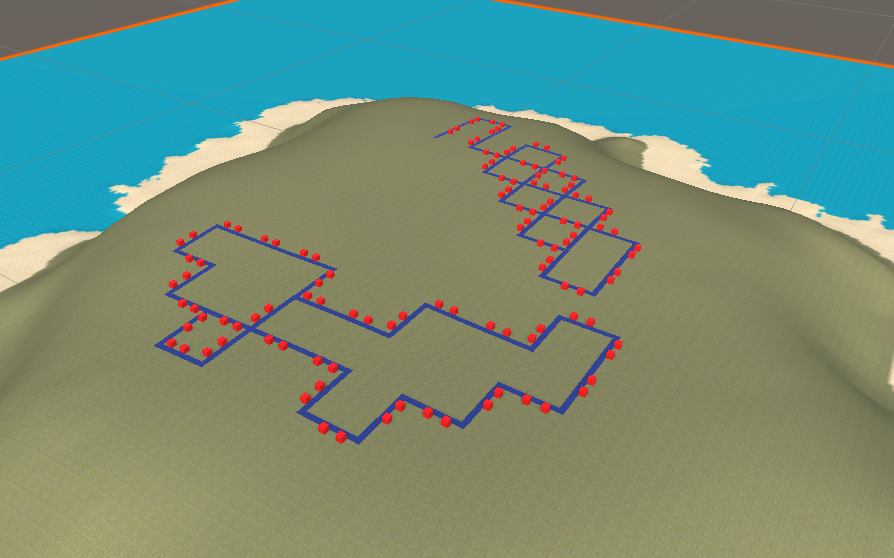
\includegraphics[width=60mm]{images/City Agent/2/3}}
    \end{figure}

    \newpage

    \section{Tree Agent}
    Tree agent works for placing tree on the landmass. In order to do that the landmass have to be quite flat, so the point considered have not to be so steep. Unless the city agent,
    this time are allowed point a bit more steep. 

    \subsection{Agent Parameter}

    \begin{itemize}
        \item \textbf{agentNr:} it is the number of agents which will place tree on the map. Every agent takes care about a specific zone of the map, generating a number of tree
        according to the parameter specified. It can happen that an agent is placed near a zone where another agent has already worked, in this case the new agent increase
        zone details.
        \item \textbf{token:} the number of token represents the number of action which an agent can perform. An action consist of placing a number of tree until the return value
        isn't reached. Of course while the agent are placing trees it move itself every time towards a random neighboring point according to distance parameter.
        \item \textbf{returnValue:} this value is used in order to let the agent don't perform a random walk around the map placing tree, but forcing it to work in a specific zone of 
        the map making it come back periodically to its starting point.
        \item \textbf{distance:} it is a range between [5, 10] which specifies the maximum distance between one tree and others. Actually, when the agent have to move itself, it uses this
        parameter in order to understand how much far it has to move, the value is chosen in random way between the lower bound and the upper bound of the chosen range.
        \item \textbf{tree:} this is the game object used as tree, it is used a real tree model.
    \end{itemize}

    \subsection{Action}
    When the action start, heightmap matrix is filled with the value related to the heights of the landmass. Then all valid points are collected using \textbf{ValidPoints} method, see
    section \ref{section:validPoints}. As it happened for city agent, it is important to retrieve world coordinate for the terrain in order to place trees in the right world point on the terrain.

    Every agent have to be placed on the map and the position will be retrieved thanks to \textbf{RandomStartingPoint} method which return random valid points
    retrieved by the one previously found. Then the agent work can start. It will return periodically to the starting point just found according to \textbf{returnValue} parameter. 

    When the agent is placed on the map it is used a variable for keeping track its position called \textbf{candidate}, at the beginning it is set to the starting point and
    every time the agent have to came back to its position it is used. At this point the agent tries to move itself to a valid near point using \textbf{GetNearbyPoint} method, see section \ref{section:nearbyPoint}.
    If a valid point is found the agent move itself to it and then place a tree, otherwise he come back to its starting point trying to find another way where to place tree. If 
    no valid points are found the agent work ends.

    Since it is used a unity coroutine every time the agent finish a walk a frame is waited, like at the end of the action.

    \subsection{Valid Points} \label{section:validPoints}
    This method is responsible to find all valid points on the landmass where it is possible to place the agent. In order to do that, like in the city agent, the first thing checked 
    is if the height of the point is grater than the average height of the landmass plus 0.05, see section \ref{section: ValidPoints}. Then the other important thing is to check the point
    steepness. The method \textbf{CheckSteepness} is used and the angle between the normal vector and the up vector is checked. This time, unless the city agent, if the angle is grater
    than 15-degree the point isn't a valid one. All map points are checked and only valid one are returned.

    \subsection{Get Nearby Point} \label{section:nearbyPoint}
    Every time the agent have to find a point where it can move itself according to distance parameter specified earlier, a random distance have to be computed between the range specified.
    Then every point, at direction specified in the \textbf{nearbyPoints} array and at random distance previously computed, is checked with \textbf{IsValidPoint} method. If the point 
    checked is a valid one it is considered. At the end, a random valid point is returned. It is possible that no valid point can be found, so it is returned the location given in input,
    in this way the agent can understand that it can't move itself to another point and ends its work.
    
    \textbf{IsValidPoint} method check if the candidate point is inside the map and if it is not too steep. When the agent have to place the tree on the map it is important that 
    the game object doesn't collide with others. This method perform also this check using \textbf{OverlapBoxNonAlloc}, since it is not needed information about collision but only
    if there is collision or not. In order to perform the previous check it is needed that the game object has a box collider attached to it, since it is used 
    as measures on how large the space to be controlled must be.

    \subsection{Results}
    Below there are some examples of the result achieved and the related configuration about parameters.

    \begin{figure}[H]
        \centering
        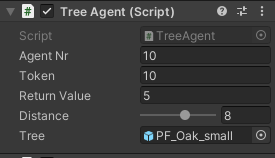
\includegraphics[scale = 0.8]{images/Tree agent/1/Parameters}
        \caption{Parameters used for the following results.}
    \end{figure}

    \begin{figure}[H]
        \centering     %%% not \center
        \subfigure[First result]{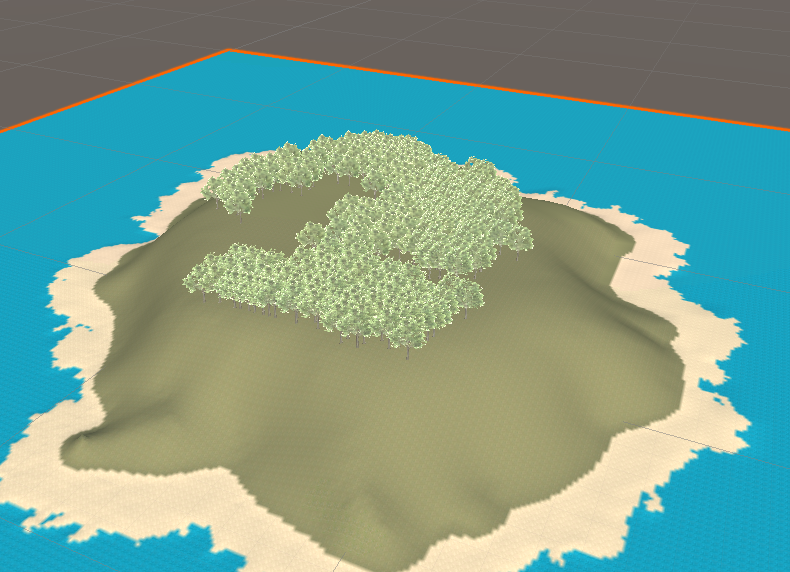
\includegraphics[width=60mm]{images/Tree agent/1/1}}
        \subfigure[Second result]{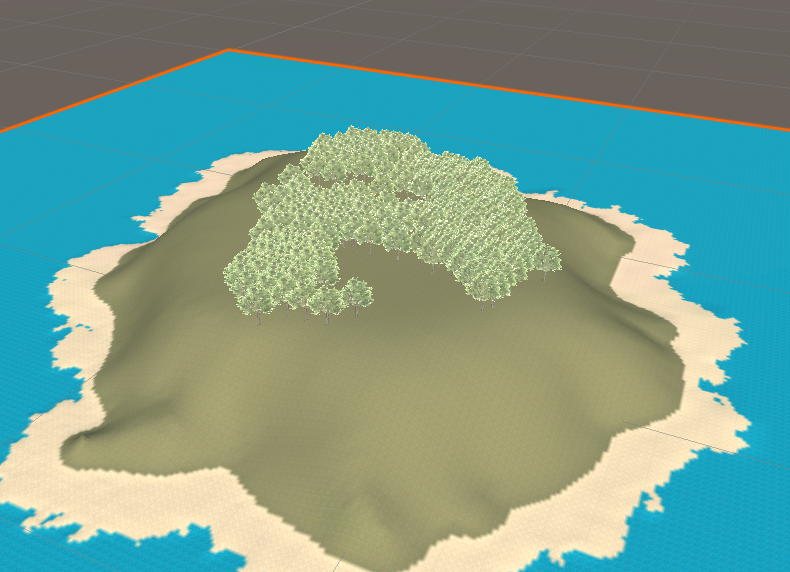
\includegraphics[width=60mm]{images/Tree agent/1/2}}
        \subfigure[]{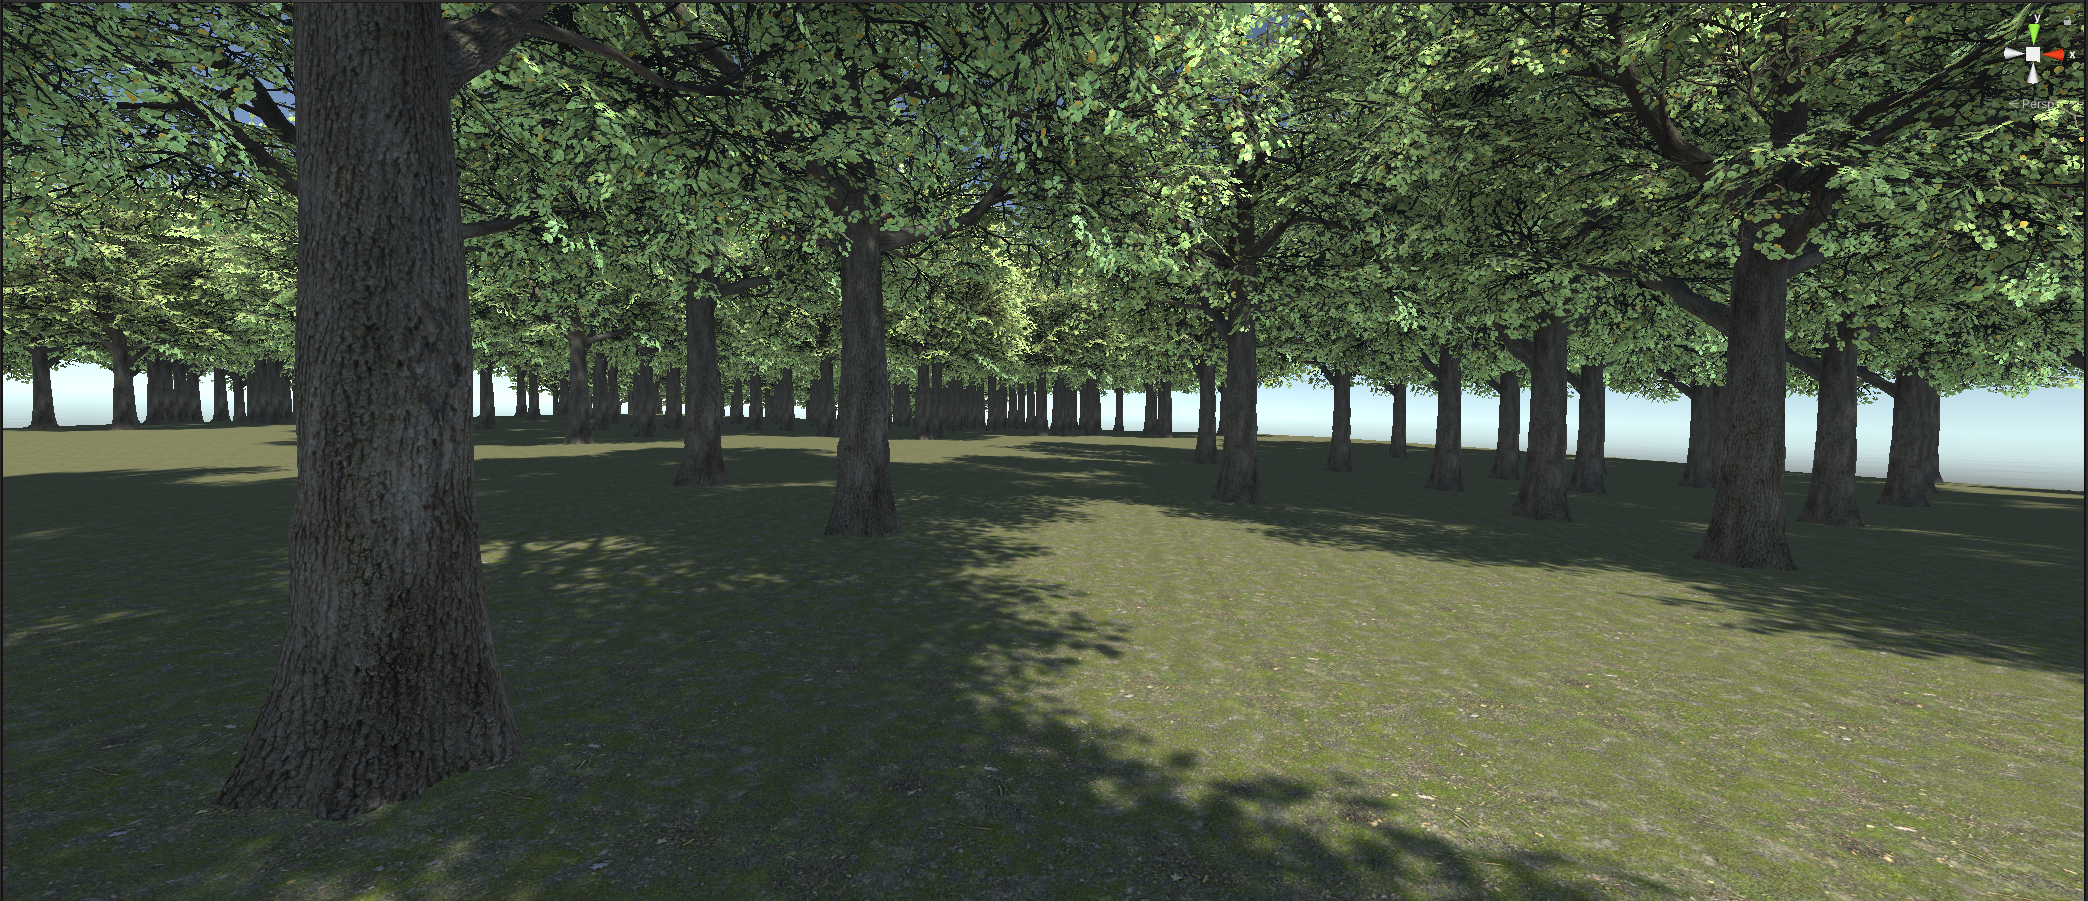
\includegraphics[width=80mm]{images/Tree agent/1/3}}
    \end{figure}

    \begin{figure}[H]
        \centering
        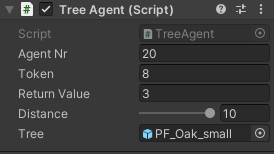
\includegraphics[scale = 0.8]{images/Tree agent/2/Parameters}
        \caption{Parameters used for the following results.}
    \end{figure}

    \begin{figure}[H]
        \centering     %%% not \center
        \subfigure[First result]{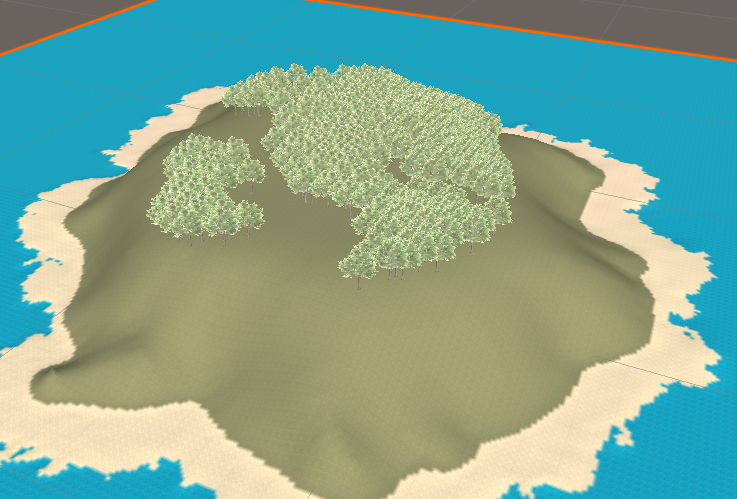
\includegraphics[width=60mm]{images/Tree agent/2/1}}
        \subfigure[Second result]{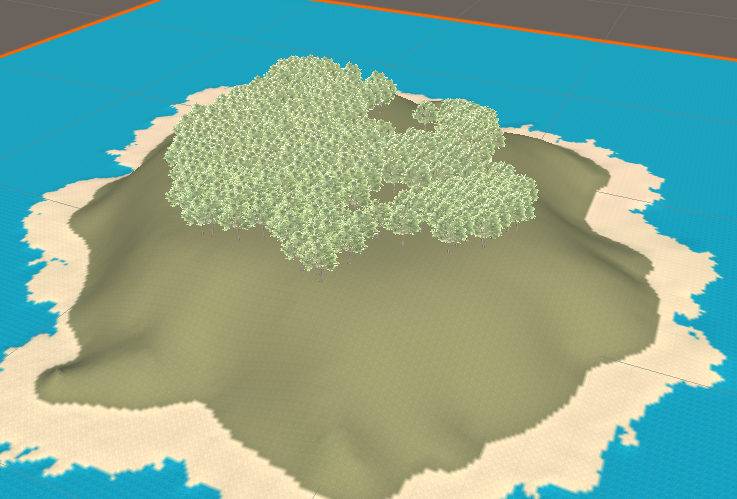
\includegraphics[width=60mm]{images/Tree agent/2/2}}
        \subfigure[]{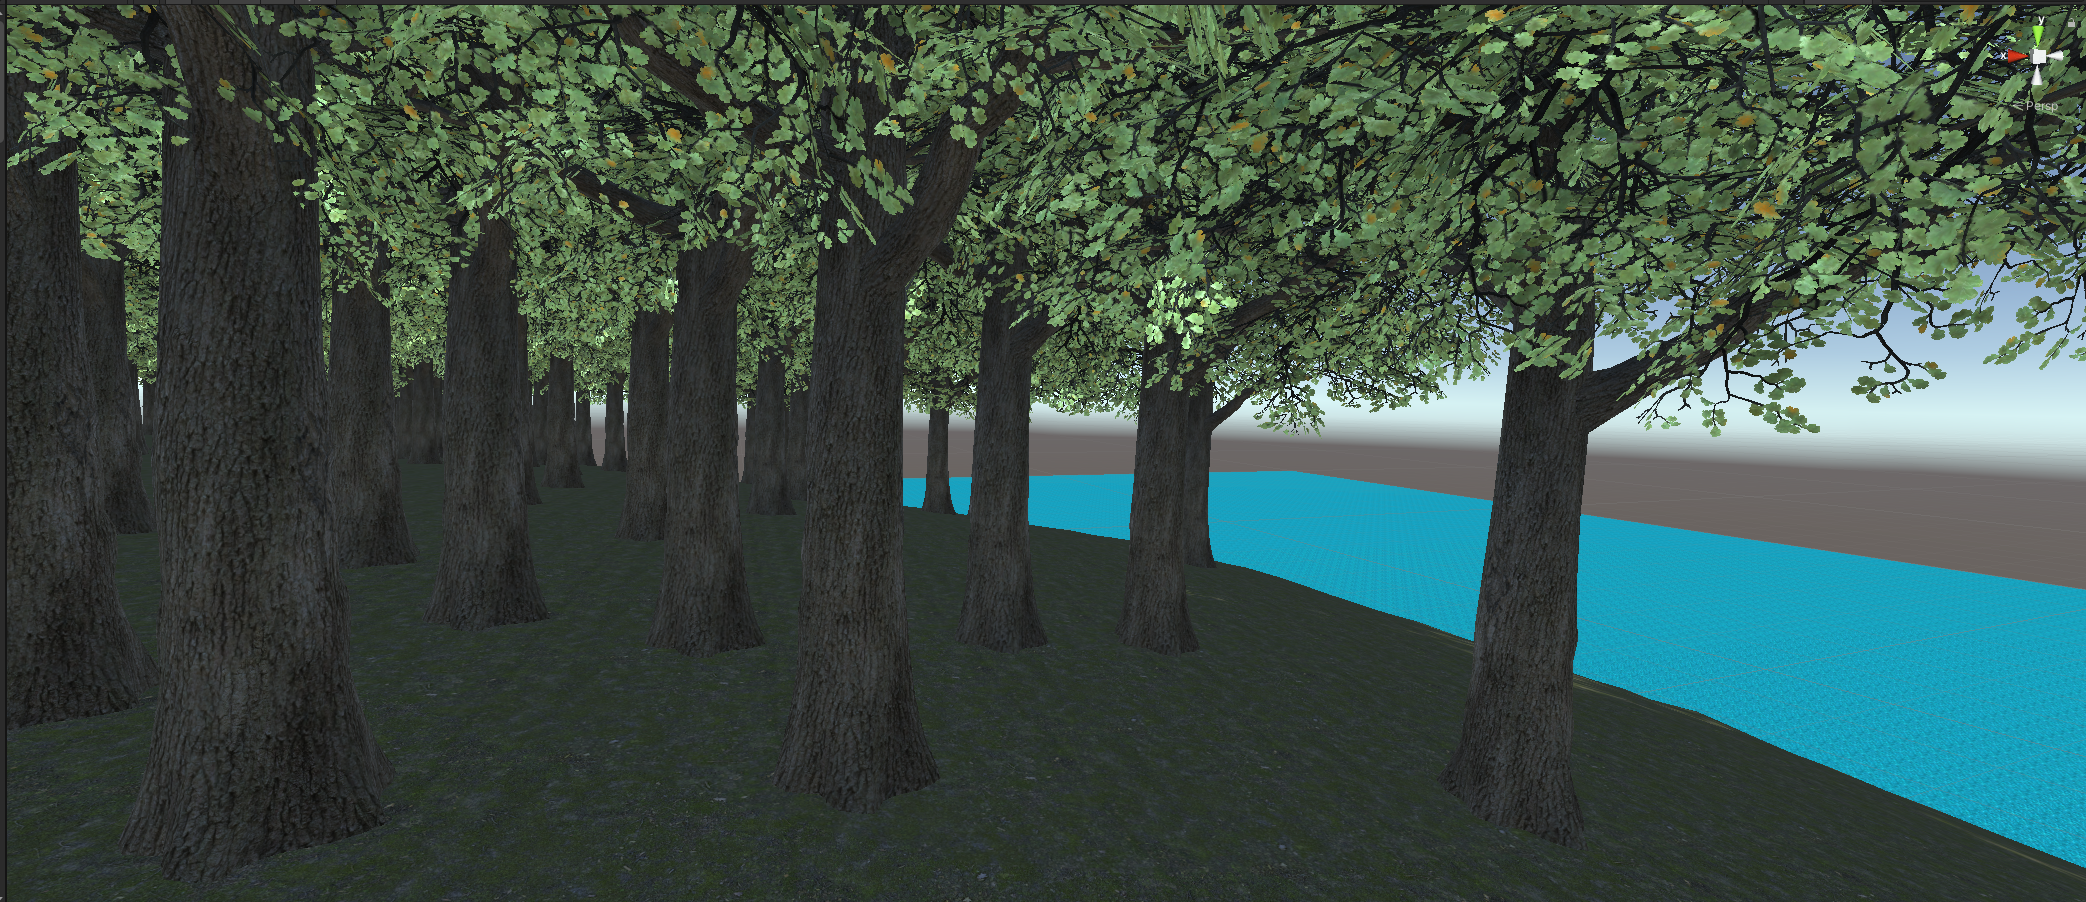
\includegraphics[width=80mm]{images/Tree agent/2/3}}
    \end{figure}

    \newpage
 
    \section{Harbor Agent}
    This agent place harbors all around the coastline according to parameters chosen. The harbors are placed at boundary between sea points and beach point. 
    
    \subsection{Agent Parameter}

    \begin{itemize}
        \item \textbf{agentNr:} represent the number of agent which will place harbor on the map.
        \item \textbf{token:} it is a value related to the number of action performable for a single agent. An action for this kind of agent consist of place a harbor 
        and move itself to another valid point along the coast.
        \item \textbf{timesSearchingPoint:} When there are few coastline points where it is possible to place harbor, or when the number of harbor to be placed is bigger than
        the number of point available, it can happen that the agent isn't able to find a point where it is possible to place a harbor. So in this case, the designer can
        decide how many times the agent can try to find a valid point.
        \item \textbf{distance:} it is a range between [5, 50] which represent the minimum distance between two harbors. When the agent have to find another valid point,
        it moves itself according to this parameter. The agent just move itself through the point until it visited at least a number of point equal to the value of this parameter. 
        \item \textbf{harborLenght:} this is a range between [5, 15] which represents the maximum value related to the length of the harbor. Its length is chosen randomly
        according to the range specified.  
        \item \textbf{harbor:} it is the game object used for representing the harbor. It is used the same prefab used by the city agent for the roads, the only different
        is the material attached on it which, this time, is gray instead of blue.
    \end{itemize}

    All the valid points are stored inside a list in order to easily retrieve them when an agent have to be placed on the map, see \ref{section:HarborValidPoints}. Then the 
    agent have to move itself to the near valid point, but it is needed to avoid coming back to previously visited points and in order to do that it is used another list
    for keeping track these points related to a single agent.
    
    \subsection{Action}
    The first thing done is retrieving all valid point thanks to the \textbf{ValidPoints} method, see \ref{section:HarborValidPoints}. Then it is tried to find a point where it is possible to
    place the agent using \textbf{GetStartingPoint} method, see section \ref{section:harborStartingPoint}. If it is impossible to find point means that no more points are available to place
    the harbor, so the agent work ends. If a point is found the first harbor is placed. The agent have to move itself following the coast, for this an attractor and a repulsor
    point are used for scoring the best point in which to move, see section \ref{section:attractor}.
    
    Since the first harbor is usually placed when the agent is placed on the map, the agent have to place a number of harbors equal to the number of tokens minus 1. Then a 
    location where the agent can move is searched. If it is found, a harbor is placed, otherwise a placeholder value is returned in order to communicate that near valid points
    isn't available, so the agent is moved to a random coastline point.

    After an agent ends its work, the list used for keeping track of the already visited points is clean, since it is related to a single agent.

    \subsection{Valid Points} \label{section:HarborValidPoints}
    A valid point is a point where its height is greater than 0.03 and if there is at least one near point which respect some constraints, these are checked thanks to
    \textbf{CheckNearPoint} method. This method check if the point given in input is inside the terrain and if its height is less than 0.03. In this way, it is possible to
    retrieve all the beach points which are next to a sea point.

    \subsection{Get Starting Point} \label{section:harborStartingPoint}
    This method receive in input a list of Vector2 called candidates in order to understand if the nearby points are valid ones, see seciton \ref{section:harborNearby}. Since the list 
    used is a list of object the value are in the heap, so it is not needed to return this as parameter in order to preserve the value.

    The first thing done is to retrieve a random coastline location using the method \textbf{RandomPoint} which return a random point from the coastline points list previously
    filled, see section \ref{section:HarborValidPoints}. If the location is a good one it is returned, otherwise it is retrieved another random coastline point until a good
    location is found or the number of time which is possible to try to find a point (specified by \textbf{timesSearchingPoint} parameter) is expired.
    This check is done using \textbf{CheckLocation} method, see section \ref{harbor:checkLocation}. At the end, If no point is found a placeholder value is returned in order 
    to communicate that it isn't possible to find a valid starting point.

    \subsection{Check Location} \label{harbor:checkLocation}
    This method is used for checking if the location given in input is a good location where to place a harbor or not. The first thing to check is whether, in a squared area
    as big as the harbor length, there is another harbor or not, if it is, the point considered is not a valid one. Then it is needed to check all surrounding point of the 
    one given in input and try to find a direction in which is possible to place the harbor, see section \ref{section:harborNearby}.

    Here, the list which represents the candidate points is filled with the valid surrounding points of the location given in input, if there are. It is not needed to return it,
    since it is located on the heap and its values are preserved. 
    
    \subsection{Check Nearby Point} \label{section:harborNearby}
    This method receives two input, the location and a candidate point which is one of the points surrounding location called candidate. The first thing checked is
    if the candidate is a sea point, so if its height is equal to 0. In order to place the harbor, it is important to check all the point along the direction defined by those
    two point and their right and left points. The number of points to check along that direction are equal to the maximum harbor length, since at this time the length for 
    a harbor isn't decided yet.

    For every point along the direction it is checked if the point is inside terrain, if it is a sea point and if its right and left points are a sea one. This is done
    retrieving the information about their height. The last thing checked is if there is already another harbor placed along the direction previously mentioned.
    % This list is 
    % used by every method which uses this, actually they are \textbf{FindNewLocation} (see section \ref{section:harborNew}) and \textbf{GetStartingPoint} (see section \ref{section:harborStartingPoint}).

    \subsection{Find New Location} \label{section:harborNew}
    It takes in input the location, attractor and repulsor point. The agent have to move itself through a number of points according to \textbf{distance} parameter. In order
    to do that every time it tries to move itself to a nearby point using \textbf{NewLocation} method, see section \ref{section:HarborNewLocation}. If it is able to move itself to a
    nearby point the new point visited is added to the related list for keeping track of it, otherwise the agent is moved to another random beach point near the sea, hoping
    it is retrieved a good one.

    After the agent moved itself through a number point related to the parameter previously specified, it is possible that the point found isn't a valid one since it can be another
    harbor near the point found or there is no valid direction where to place it. In this case, the agent keep searching for a valid point according to \textbf{timesSearchingPoint}
    parameter. If the agent find a point where it is possible to place harbor, it is placed thanks to \textbf{PlaceHarbor} method, see section \ref{section:PlaceHarbor} and the 
    point found is returned. If, during agent movement, it is unable to move itself to a nearby point it is moved to a random point and a walk is performed trying to find a 
    good point. 

    At the end if no point is found means that points available where to place harbor are very few or there none at all. So a placeholder value is returned for communicate this.

    \subsection{New Location} \label{section:HarborNewLocation}
    This method is used for retrieve a surrounding point related to the location given in input exploiting attractor and repulsor point. A surrounding point is a valid one if
    it is inside the terrain, if its height is greater or equal than 0.03, if it is a beach point next to the sea and if it isn't a point already visited by the agent.
    The third check is done using \textbf{CheckNearPoint} method, see section \ref{section:harborStartingPoint}. 

    If not a single point is found the agent isn't able to move itself, so a placeholder value is returned in order to communicate that. Otherwise, all candidates point found must
    be scored, see section \ref{section:attractor}. Then the point with the highest score is returned.

    \subsection{Attractor, repulsor and how to score} \label{section:attractor}
    The \textbf{GetAttractor} method is the one responsible to retrieve the attractor point, it easily returns a random point inside the map. Since attractor and repulsor point
    have to be in different direction, \textbf{GetRepulsor} retrieve a random point inside the map and check if its direction is different from the attractor one. While they have 
    the same direction, a new random repulsor point is retrieved. The direction previously mentioned are the one from location to the attractor/repulsor.

    Those two point are used for scoring candidate points, so the points closer to the attractor are scored higher than the ones closer to the repulsor. A point is scored 
    according to the following rule:

    \begin{equation}
        score = d(p, r)^2 - d(p, a)^2
    \end{equation}

    \noindent
    Where d(p, r) is the distance between the point and the repulsor and d(p, a) is the distance between the point and the attractor.

    \subsection{Place Harbor} \label{section:PlaceHarbor}
    This method takes in input the location where to place the harbor and a nearby sea point in order to calculate a direction useful for harbor rotation.
    
    The first thing done is to retrieve the world coordinate for the points given in input, so the location and the candidate. Then a direction from the location to the 
    candidate is calculated as well as the rotation using \textbf{Quaternion.LookRotation} which inputs are the direction just mentioned and the vector up. A random value 
    related to the harbor length is computed and with this value the scaling vector is created. At the end the harbor is instantiated at world coordinate of location with 
    the rotation previously computed, then it is scaled and translated by half of its length forward. This is done because the center of the harbor is at middle of the game
    object, so in order to avoid placing half harbor on the beach.

    \subsection{Results}
    Below there are some examples of the result achieved and the related configuration about parameters.

    \begin{figure}[H]
        \centering
        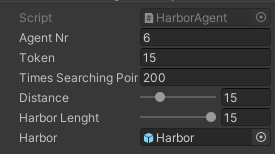
\includegraphics[scale = 0.8]{images/Harbor agent/Parameters 1}
        \caption{Parameters used for the following results.}
    \end{figure}

    \begin{figure}[H]
        \centering
        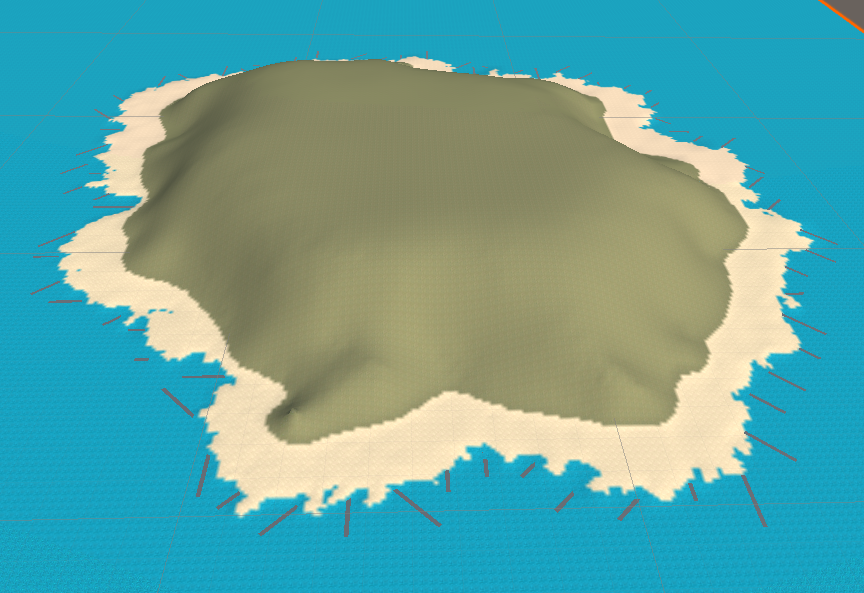
\includegraphics[scale = 0.3]{images/Harbor agent/1}
        \caption{First result.}
    \end{figure}

    \begin{figure}[H]
        \centering
        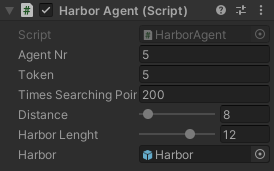
\includegraphics[scale = 0.8]{images/Harbor agent/Parameters 2}
        \caption{Parameters used for the following results.}
    \end{figure}

    \begin{figure}[H]
        \centering
        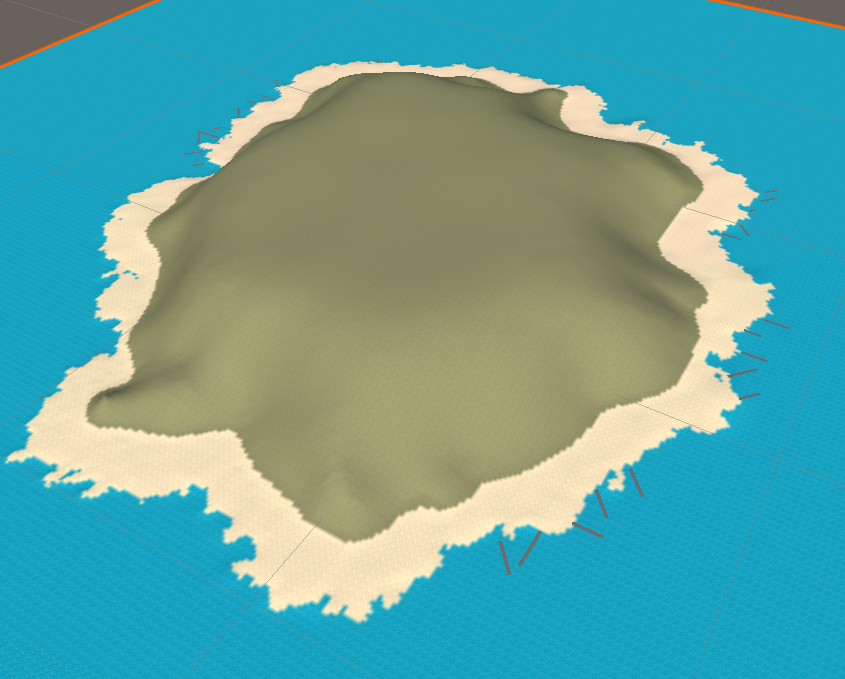
\includegraphics[scale = 0.3]{images/Harbor agent/2}
        \caption{Second result.}
    \end{figure}

    \newpage

    \section{Overall Results}
    In this section there are some result obtained after all agents have finished their work.

    \begin{figure}[H]
        \centering     %%% not \center
        \subfigure[]{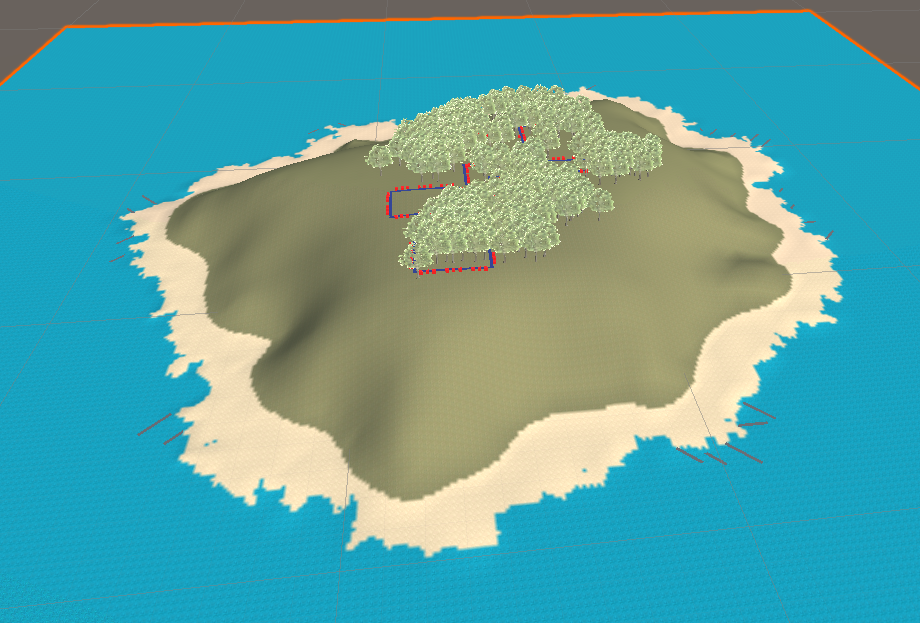
\includegraphics[width=60mm]{images/Overall/1/1}}
        \subfigure[]{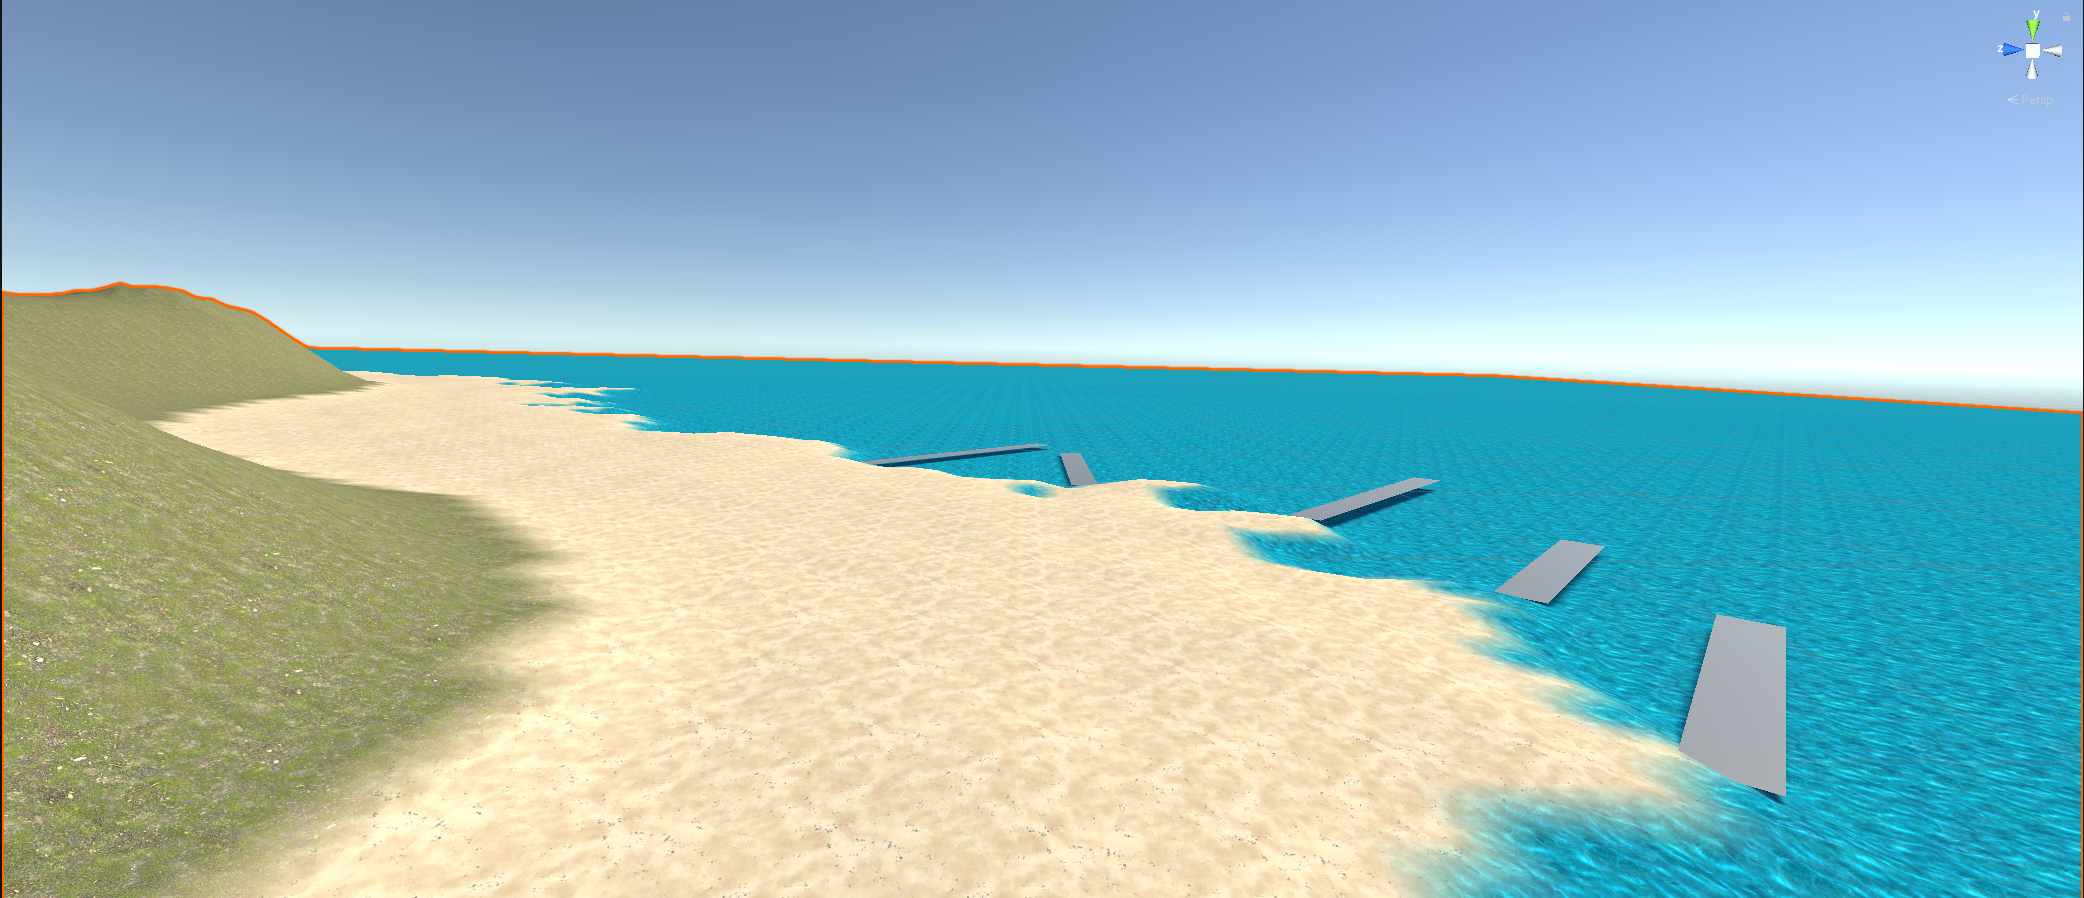
\includegraphics[width=60mm]{images/Overall/1/2}}
        \subfigure[]{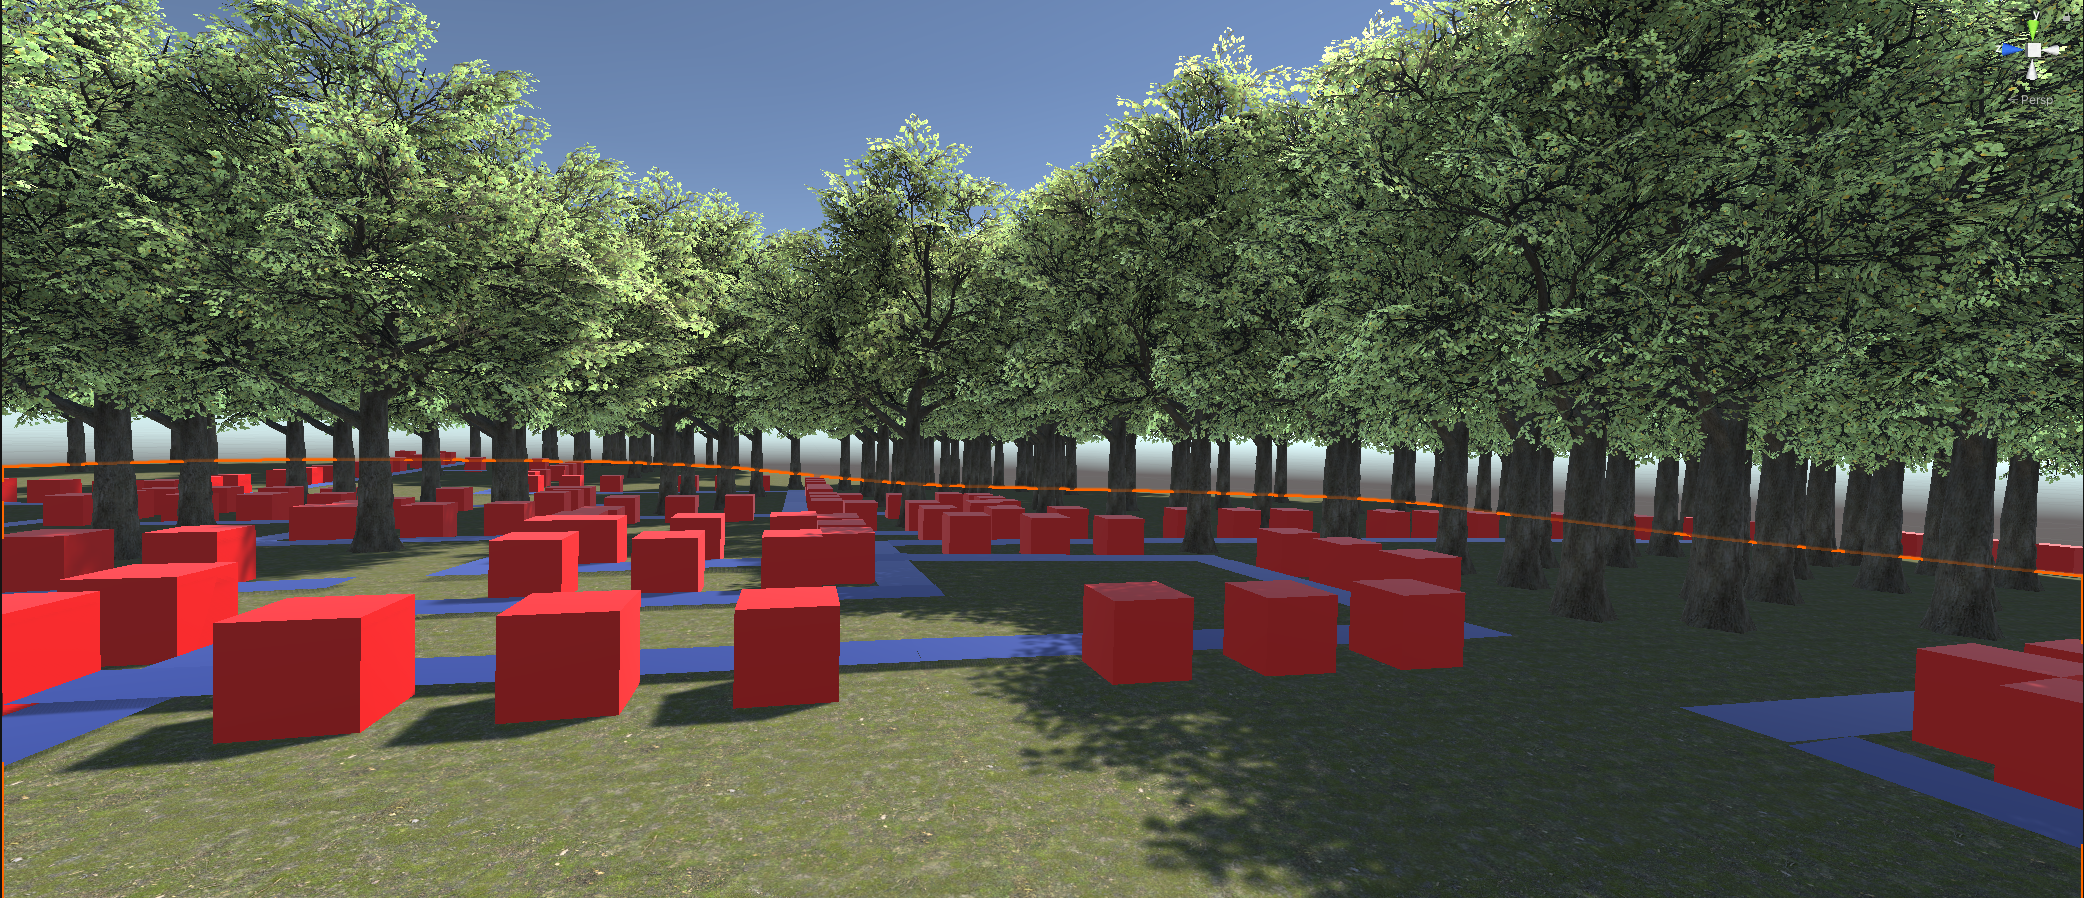
\includegraphics[width=60mm]{images/Overall/1/3}}
        \subfigure[]{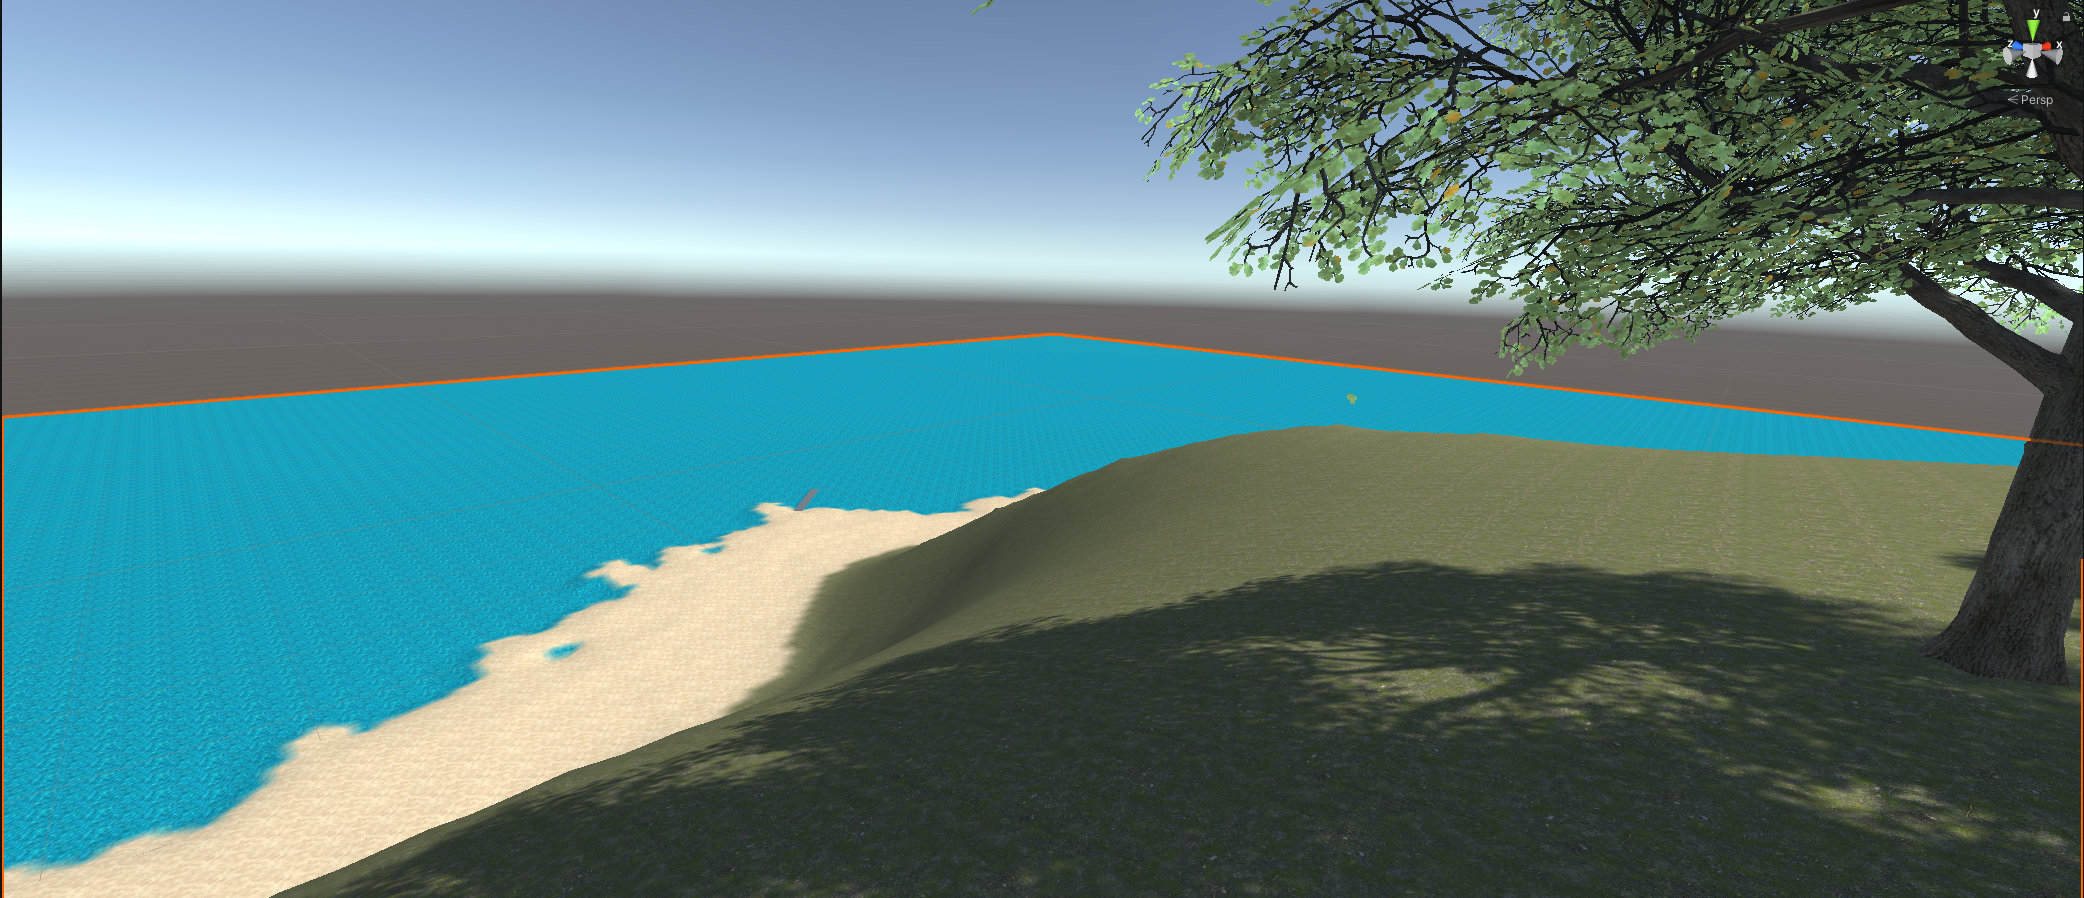
\includegraphics[width=60mm]{images/Overall/1/4}}
    \end{figure}

    \begin{figure}[H]
        \centering     %%% not \center
        \subfigure[]{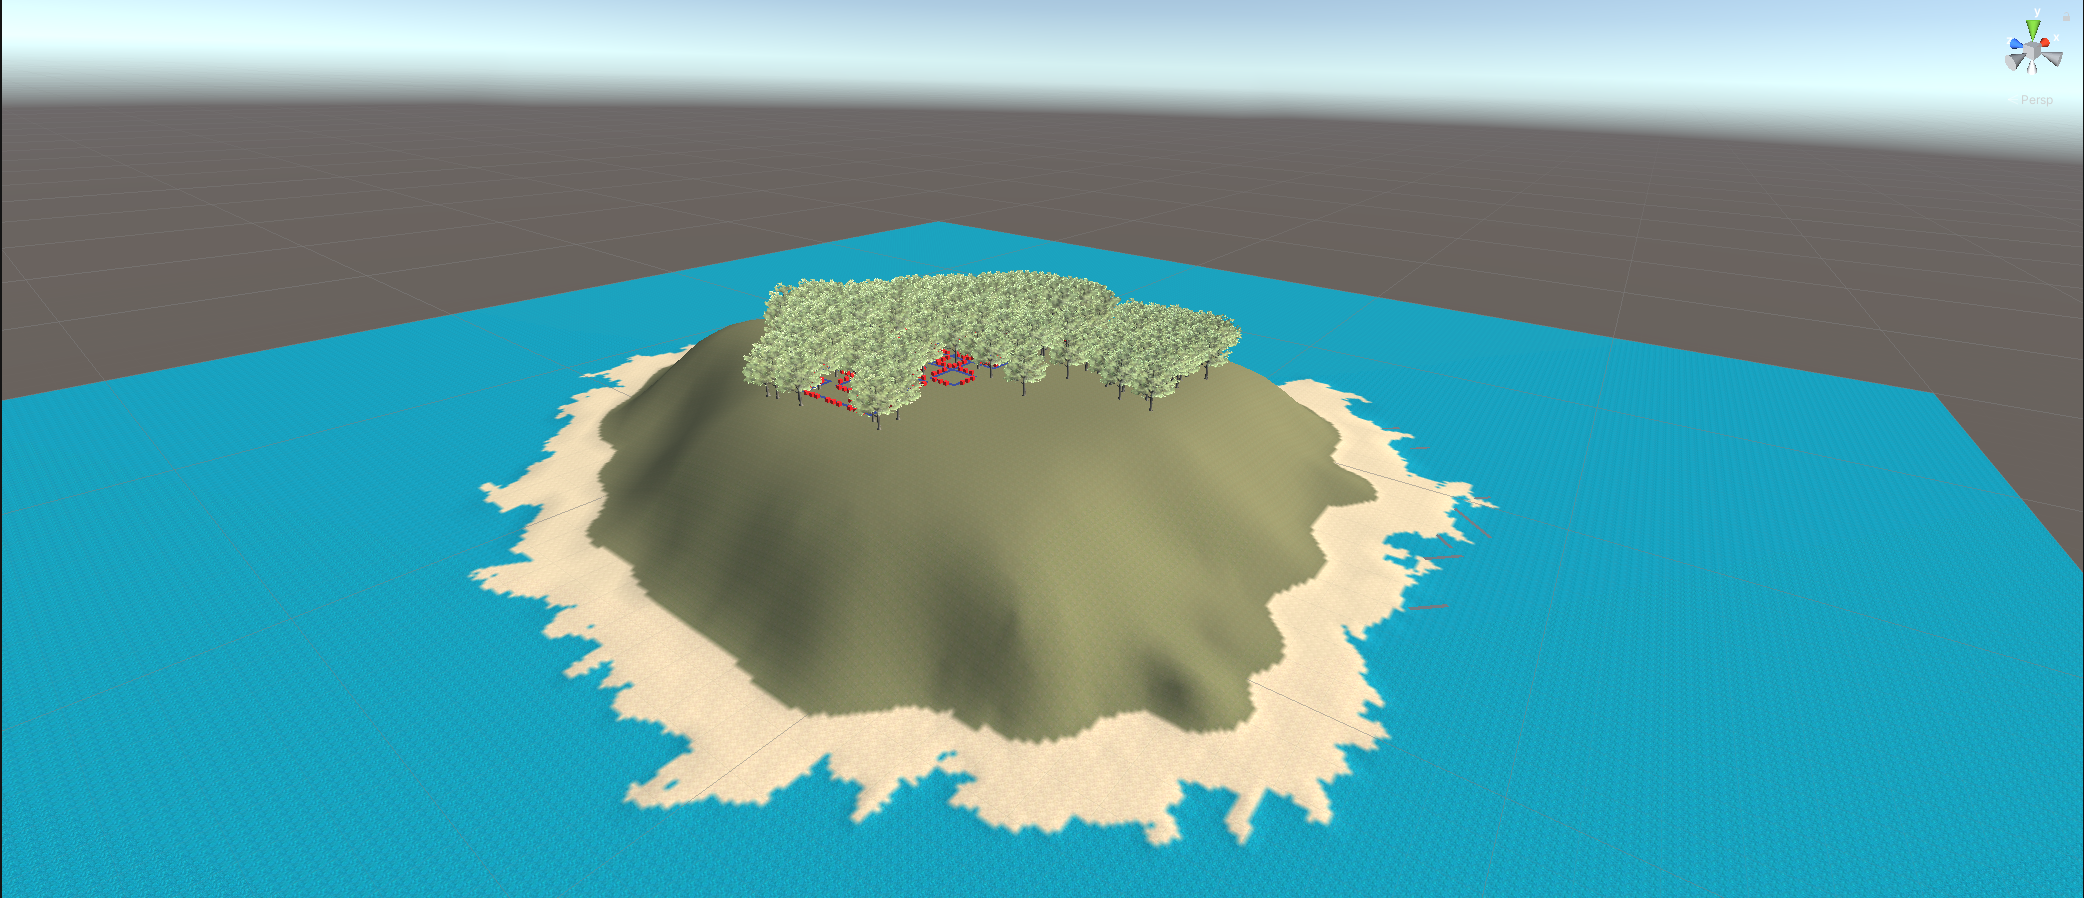
\includegraphics[width=60mm]{images/Overall/2/1}}
        \subfigure[]{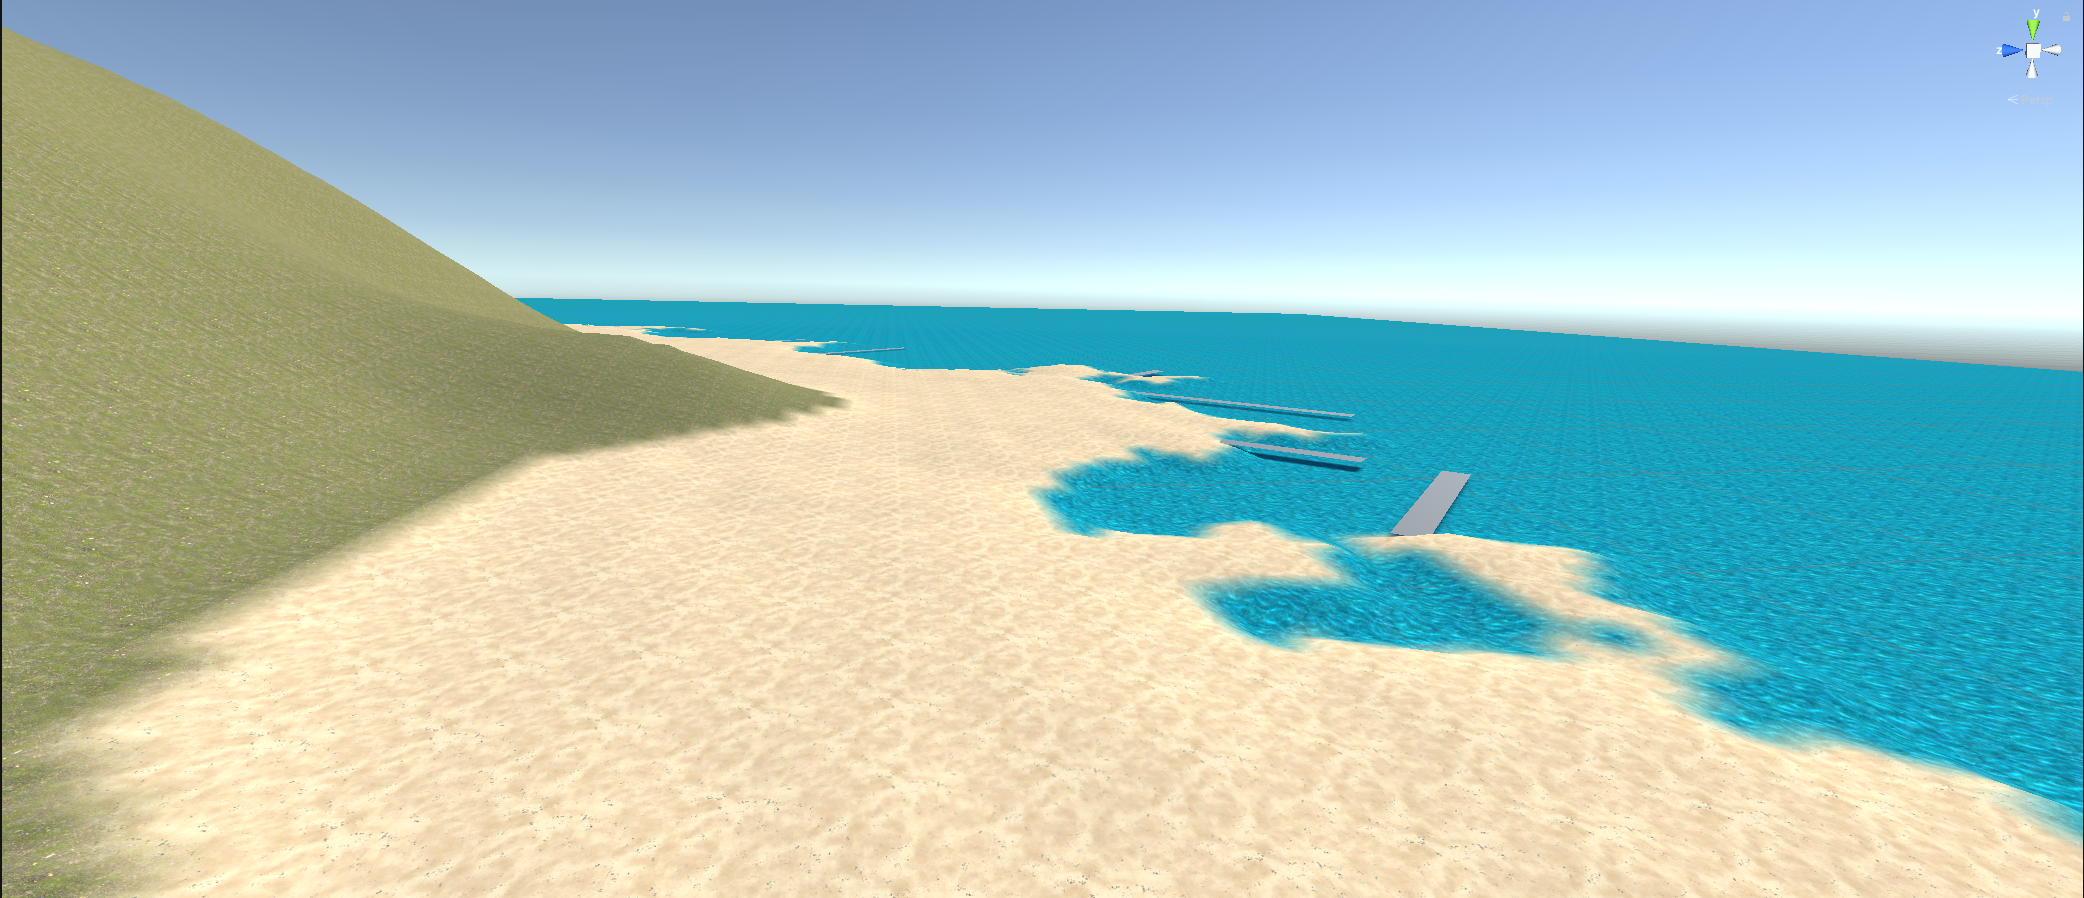
\includegraphics[width=60mm]{images/Overall/2/2}}
        \subfigure[]{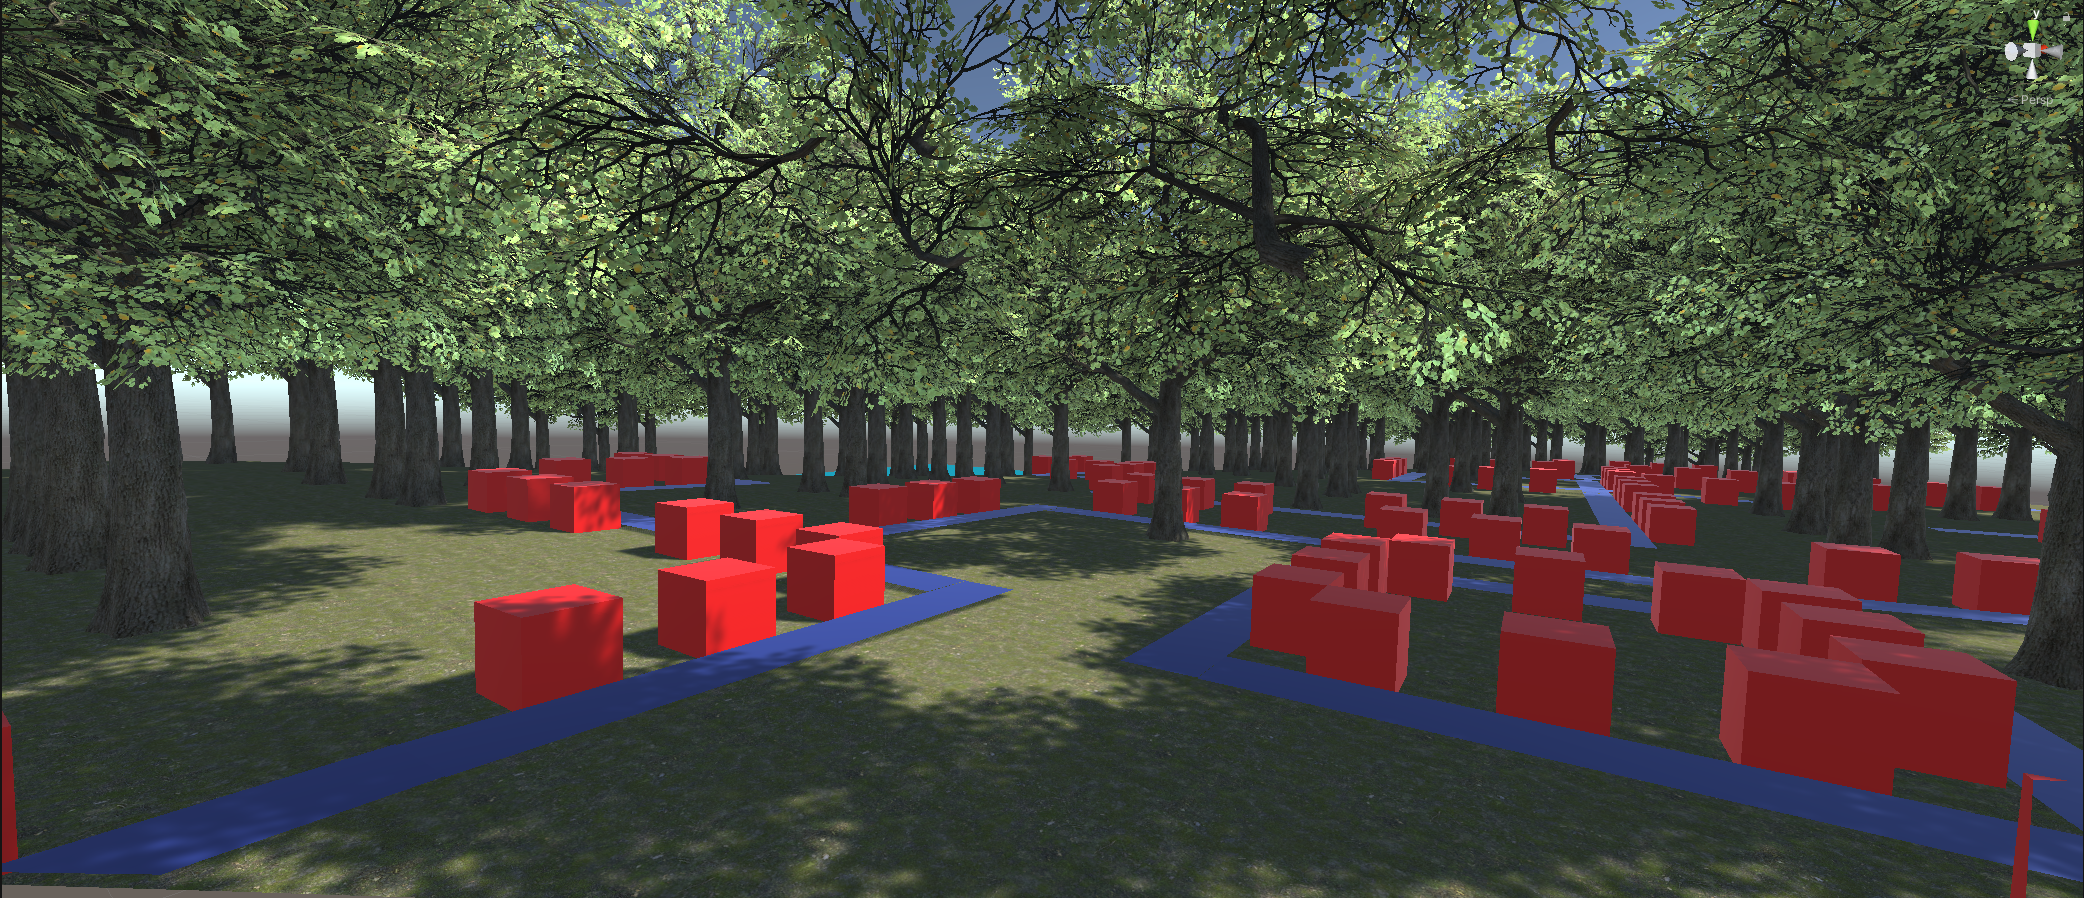
\includegraphics[width=60mm]{images/Overall/2/3}}
        \subfigure[]{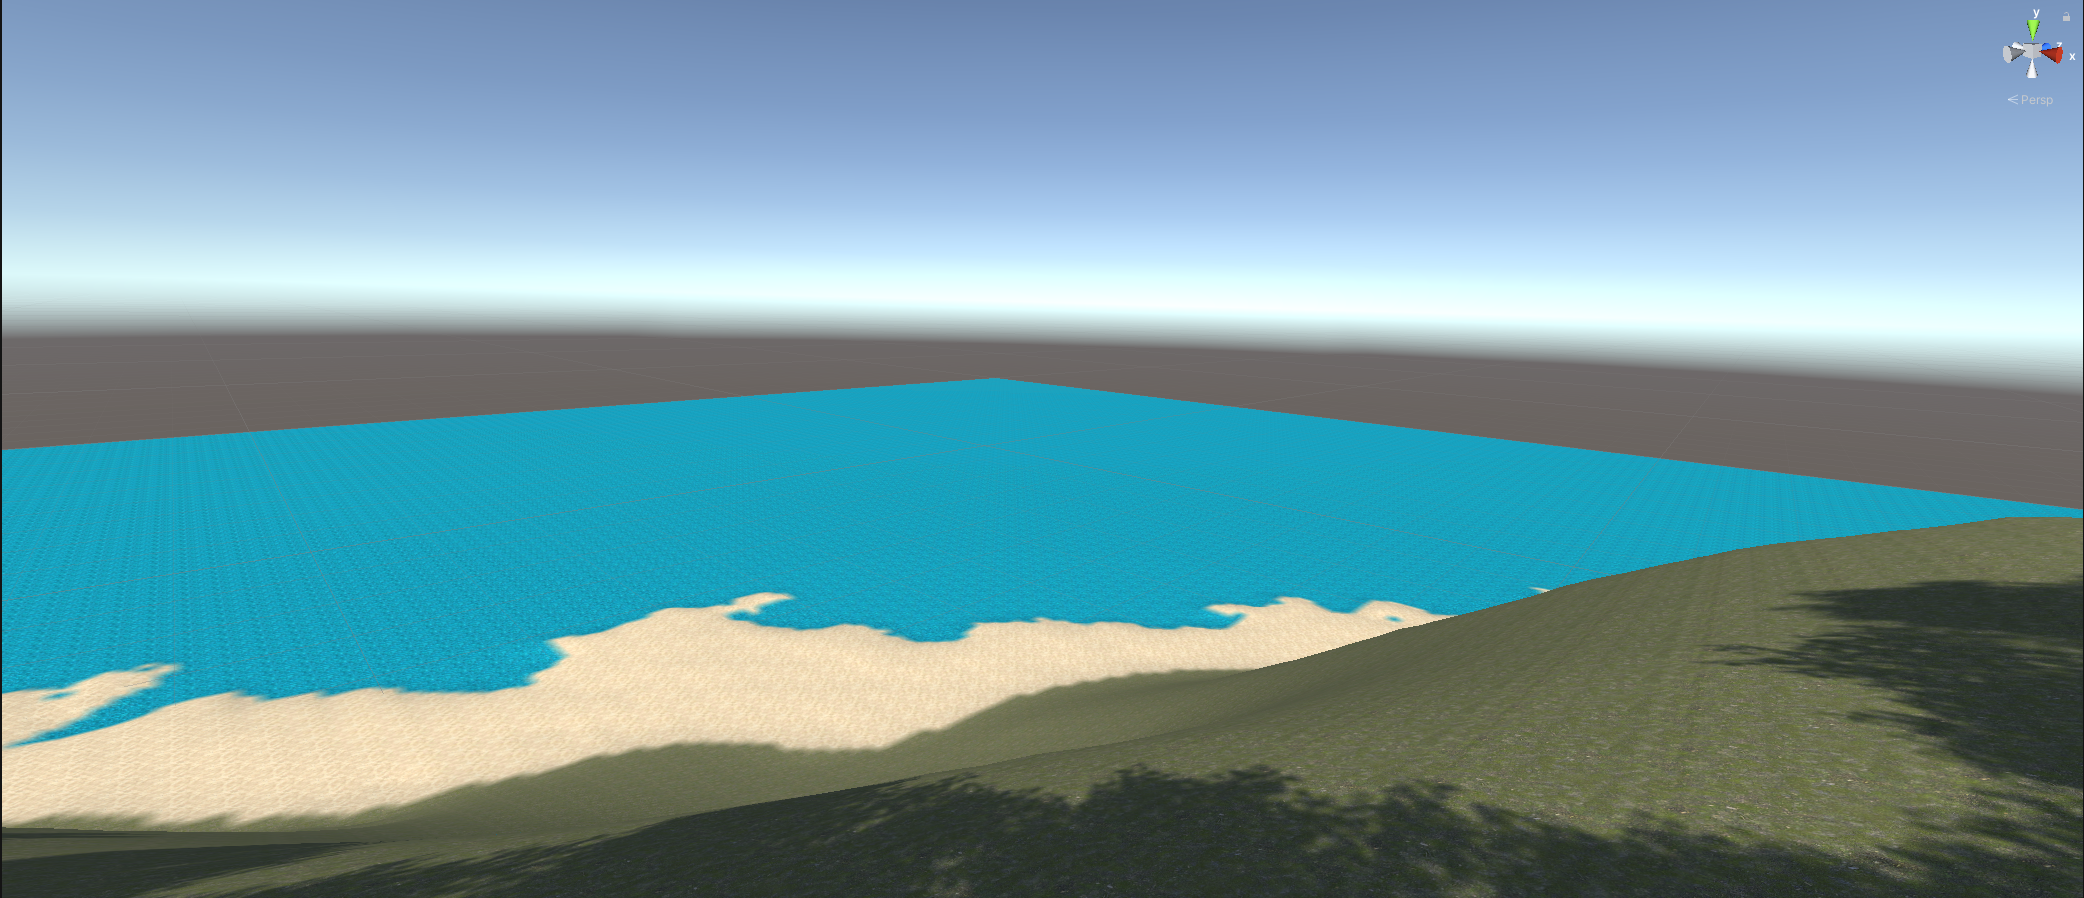
\includegraphics[width=60mm]{images/Overall/2/4}}
    \end{figure}

    \begin{figure}[H]
        \centering     %%% not \center
        \subfigure[]{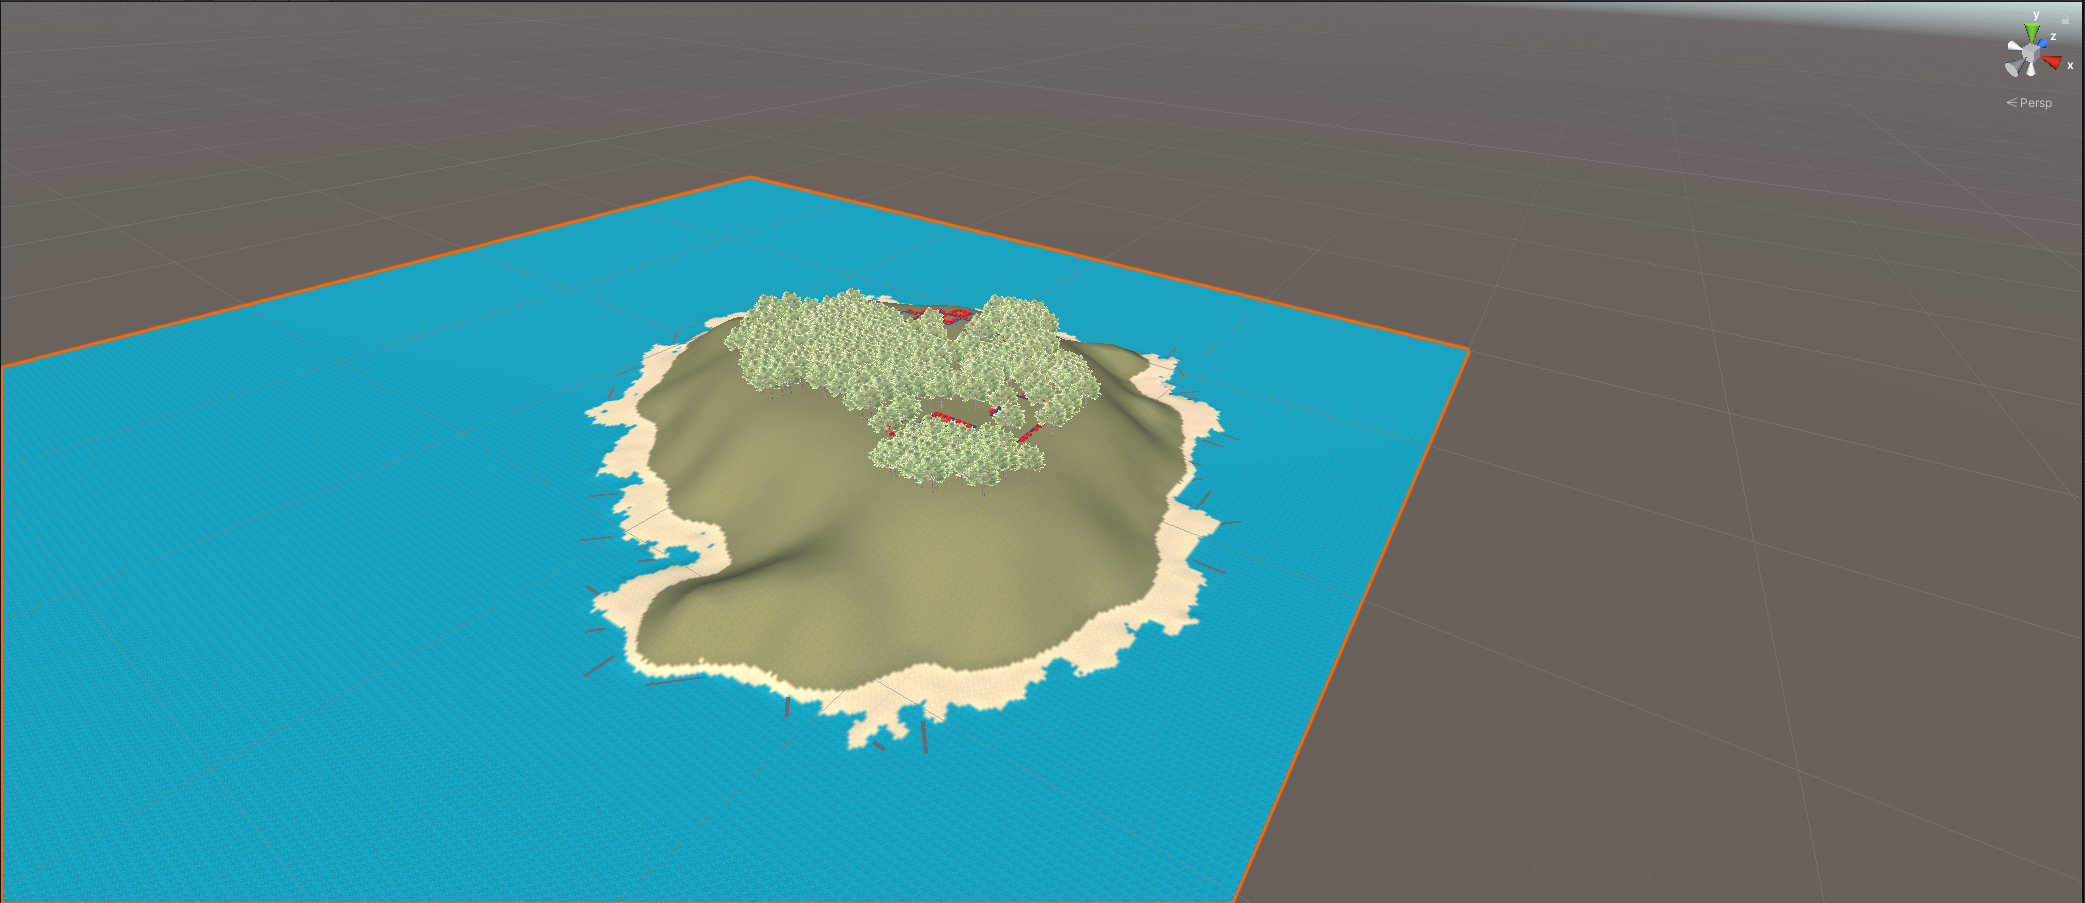
\includegraphics[width=60mm]{images/Overall/4/1}}
        \subfigure[]{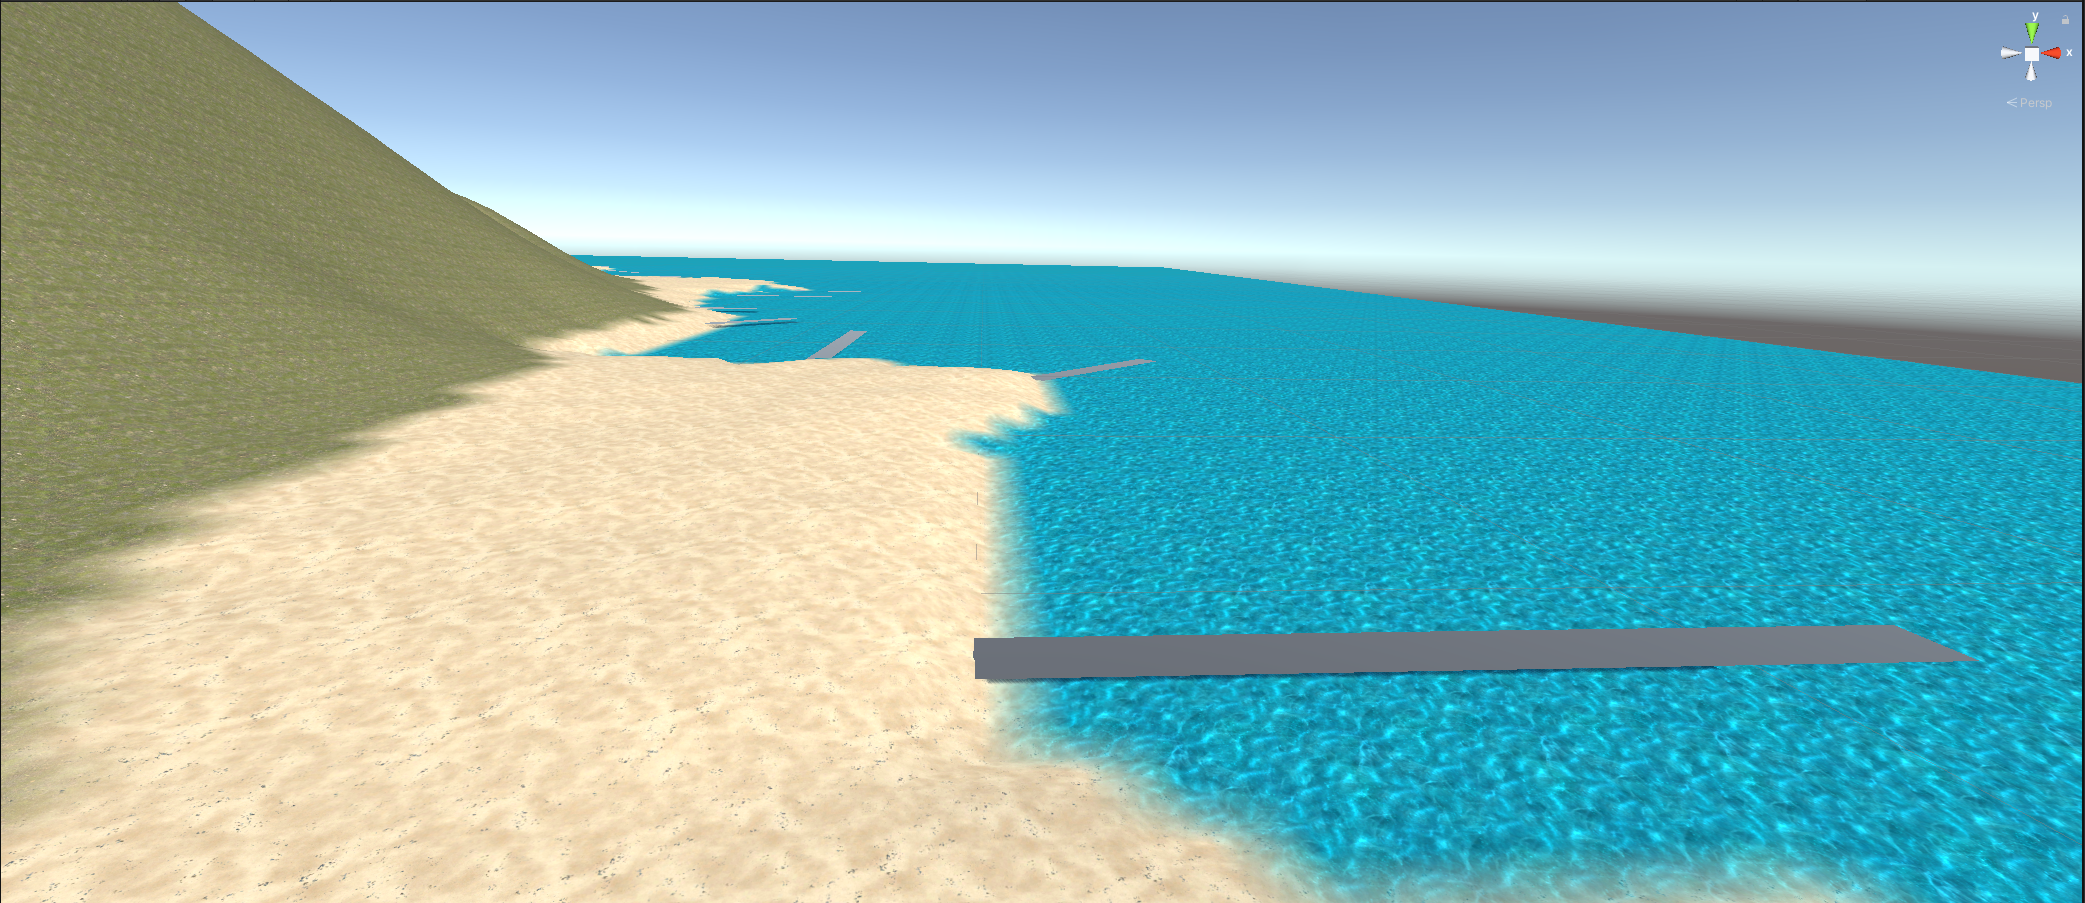
\includegraphics[width=60mm]{images/Overall/4/2}}
        \subfigure[]{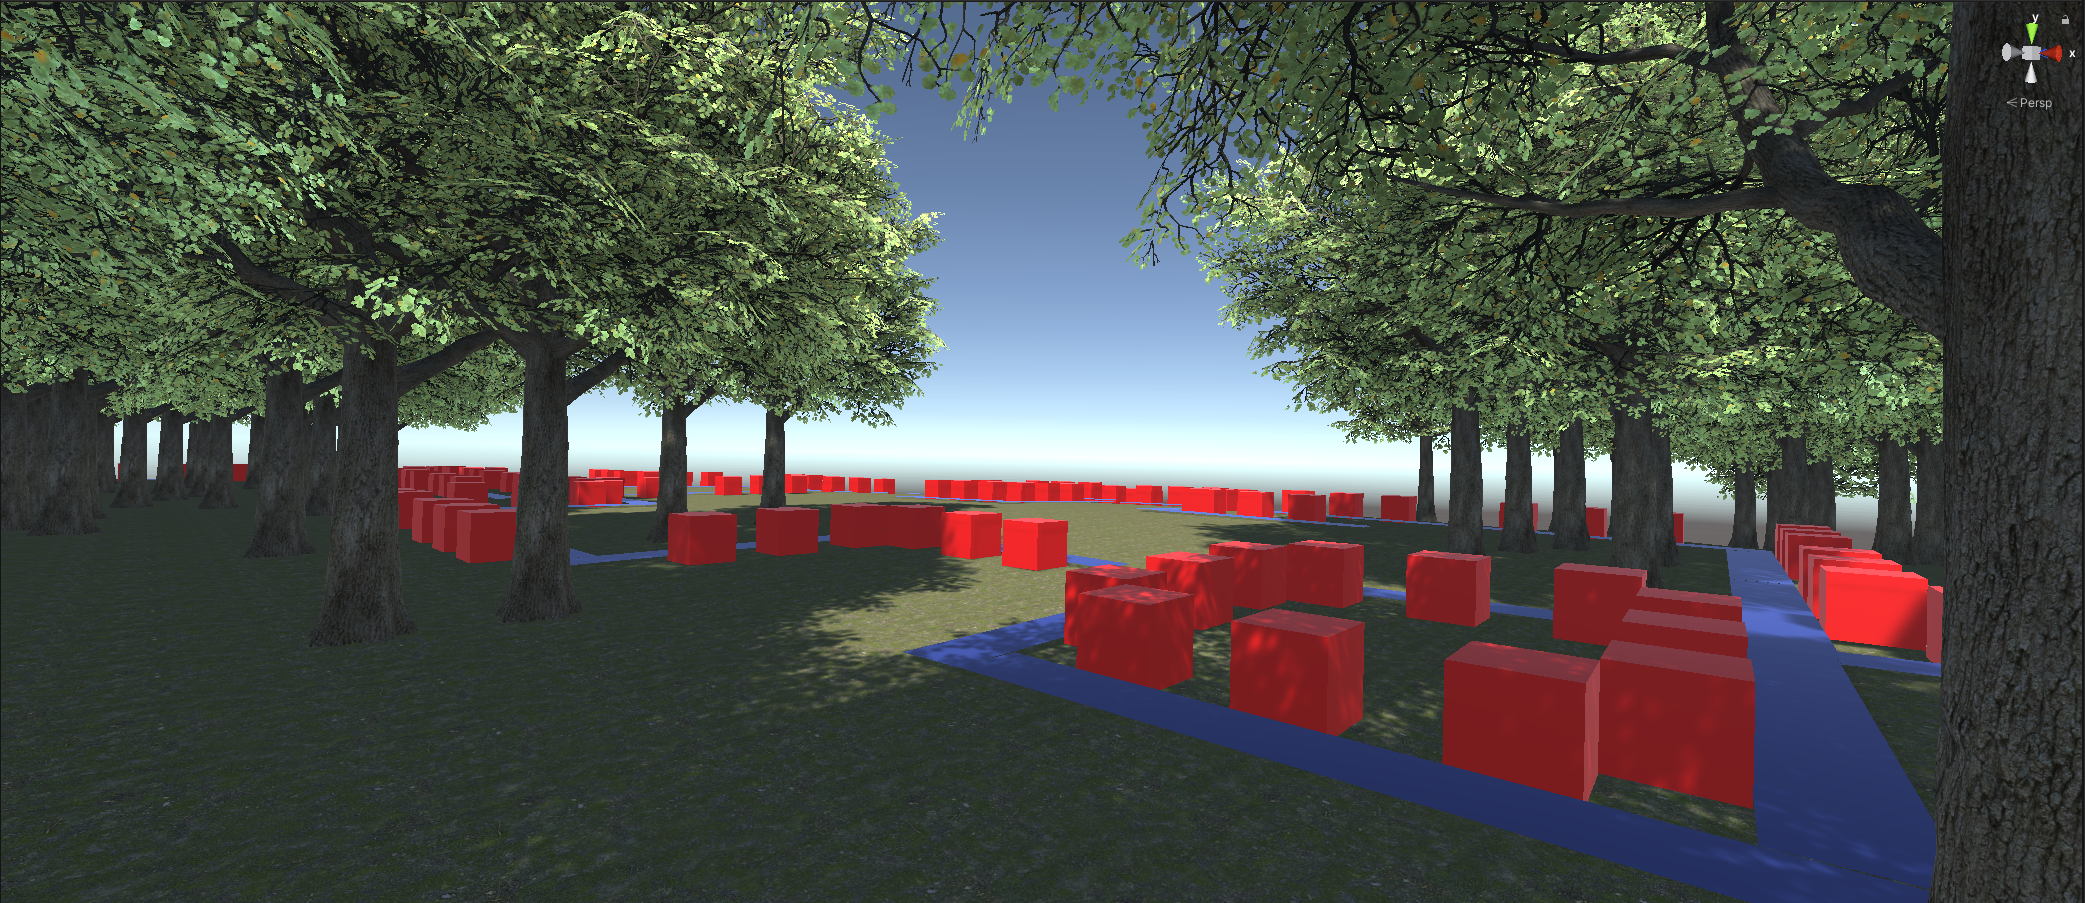
\includegraphics[width=60mm]{images/Overall/4/3}}
        \subfigure[]{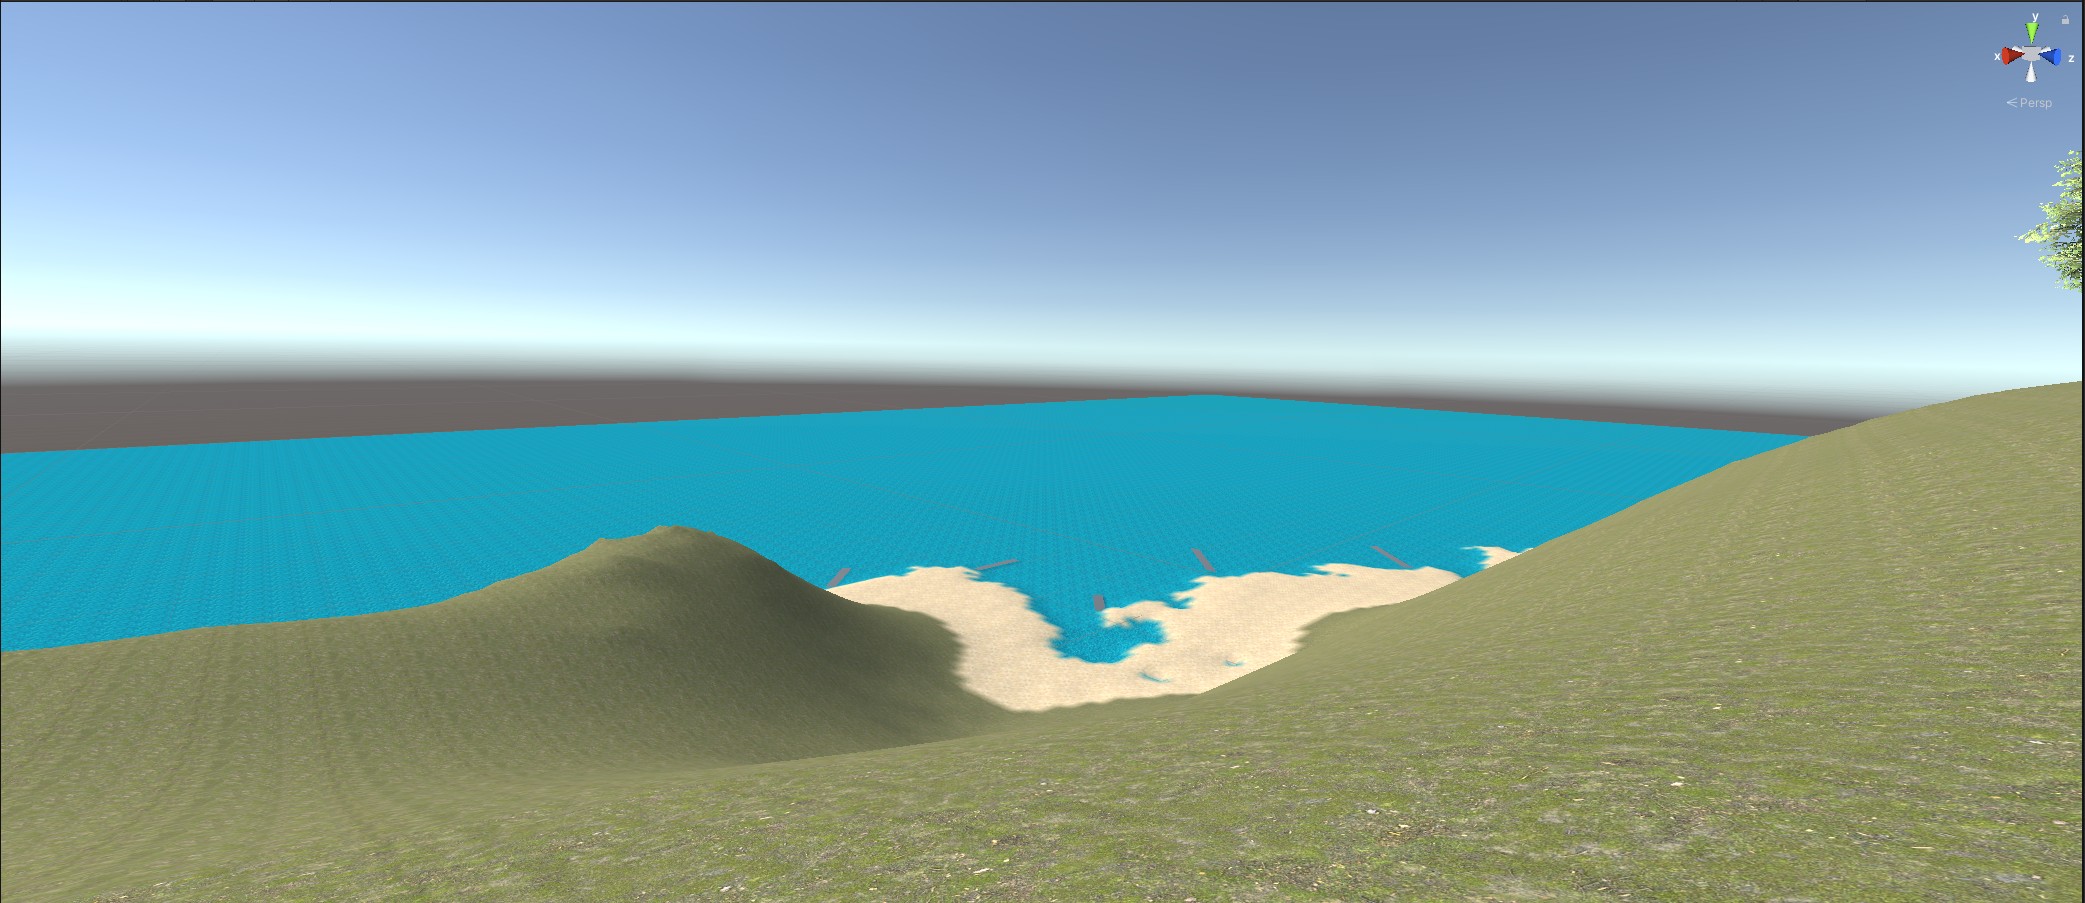
\includegraphics[width=60mm]{images/Overall/4/4}}
    \end{figure}

    \newpage

    \section{Future Improvements}
    One of the possible improvements is to implement all the possible agent already present in the Jonathon Doran and Ian Parberry's work,
    see \\ \cite{article}.
    
    It is possible to improve the city agent letting it not only create straight or perpendicular roads, but roads with different angle between each
    others. Another improvement can be to link different zone created by different agent and making this an option which is possible to select by designer.

    For all the agent which add details to the map, it is an excellent improvement modify the unity editor and create a button in order to start their work. 
    Since this is a procedural terrain generator, it is a good idea to make the asset generated permanent than let them disappear after unity run is done.
    In this way the designer can modify the asset generated adding some details or change it in a better way.

    At the end it is possible to add a lot of different agents, like the one presented in this document, capable of adding details to the map generated. 

    \newpage
    \bibliographystyle{unsrtnat}
    \bibliography{bibliography.bib}

\end{document}